\documentclass{article}


\usepackage{arxiv}

\usepackage[utf8]{inputenc} % allow utf-8 input
\usepackage[T1]{fontenc}    % use 8-bit T1 fonts
\usepackage{hyperref}       % hyperlinks
\usepackage{url}            % simple URL typesetting
\usepackage{booktabs}       % professional-quality tables
\usepackage{amsfonts}       % blackboard math symbols
\usepackage{nicefrac}       % compact symbols for 1/2, etc.
\usepackage{microtype}      % microtypography
\usepackage{lipsum}
\usepackage{graphicx}
\graphicspath{ {./images/} }
\usepackage{amsmath}
\usepackage{multirow}
\usepackage{makecell}
\setcellgapes{5pt}
\usepackage{float}

\usepackage[toc,page]{appendix}


\makeatletter
\newcommand*{\rom}[1]{\expandafter\@slowromancap\romannumeral #1@}
\makeatother

% \title{RIGID: Random-forest-based Interpretable Generative Inverse Design of Wave-based Metamaterials}
% \title{Meeting Target Spectral Ranges with Interpretable Generative Inverse Design}
% \title{Interpretable Generative Inverse Design of Wave-Based Metamaterials with Small Data}
% \title{Tailoring Qualitative Behaviors of Wave-Based Metamaterials with Small Data}
% \title{Generating Wave-Based Metamaterials with Tailored Qualitative Behaviors Using Small Data}
% \title{Generative Inverse Design of Wave-Based Metamaterials with Interpretable Machine Learning and Small Data}
% \title{Generative Inverse Design of Optical and Acoustic Metamaterials with Interpretable Machine Learning}
\title{Generative Inverse Design of Metamaterials with Functional Responses by Interpretable Learning}


\author{
 Wei (Wayne) Chen \\
  J. Mike Walker ’66 Department of Mechanical Engineering\\
  Texas A\&M University\\
  College Station, TX 77843 \\
  \texttt{w.chen@tamu.edu} \\
  %% examples of more authors
   \And
 Rachel Sun \\
  Department of Mechanical Engineering\\
  Massachusetts Institute of Technology\\
  Cambridge, MA 02139 \\
  \texttt{rmsun@mit.edu} \\
  \And
 Doksoo Lee \\
  Department of Mechanical Engineering\\
  Northwestern University\\
  Evanston, IL 60208 \\
  \texttt{dslee@northwestern.edu} \\
  \And
 Carlos M. Portela \\
  Department of Mechanical Engineering\\
  Massachusetts Institute of Technology\\
  Cambridge, MA 02139 \\
  \texttt{cportela@mit.edu} \\
  \And
 Wei Chen \\
  Department of Mechanical Engineering\\
  Northwestern University\\
  Evanston, IL 60208 \\
  \texttt{weichen@northwestern.edu} \\
  %% \AND
  %% Coauthor \\
  %% Affiliation \\
  %% Address \\
  %% \texttt{email} \\
  %% \And
  %% Coauthor \\
  %% Affiliation \\
  %% Address \\
  %% \texttt{email} \\
  %% \And
  %% Coauthor \\
  %% Affiliation \\
  %% Address \\
  %% \texttt{email} \\
}

\begin{document}
\maketitle
\begin{abstract}
Metamaterials with functional responses, such as wave-based responses or deformation-induced property variation under external stimuli, can exhibit varying properties or functionalities under different conditions. Herein, we aim at rapid inverse design of these metamaterials to meet target qualitative functional behaviors. This inverse problem is challenging due to its intractability and the existence of non-unique solutions. Past works mainly focus on deep-learning-based methods that are data-demanding, require time-consuming training and hyperparameter tuning, and are non-interpretable. To overcome these limitations, we propose the Random-forest-based Interpretable Generative Inverse Design (RIGID), a single-shot inverse design method to achieve the fast generation of metamaterial designs with on-demand functional behaviors. Unlike most existing methods, by exploiting the interpretability of the random forest, we eliminate the need to train an inverse model mapping responses to designs. Based on the likelihood of target satisfaction derived from the trained forward model, one can sample design solutions using Markov chain Monte Carlo methods. The RIGID method therefore functions as a generative model that captures the conditional distribution of satisfying solutions given a design target. We demonstrate the effectiveness and efficiency of RIGID on both acoustic and optical metamaterial design problems where only small datasets (less than 250 training samples) are available. Synthetic design problems are created to further illustrate and validate the mechanism of likelihood estimation in RIGID. This work offers a new perspective on solving on-demand inverse design problems, showcasing the potential for incorporating interpretable machine learning into generative design and eliminating its large data requirement.
\end{abstract}


% keywords can be removed
%\keywords{First keyword \and Second keyword \and More}

%%%%%%%%%%%%%%%%%%%%%%%%%%%%%%%%%%%%%%%%%%%%%%%
\section{Introduction}
\label{sec:introduction}

Metamaterials with functional responses are engineered materials that exhibit varying properties or behaviors under different conditions. One example is metamaterials whose electromagnetic, acoustic, or elastic wave propagation behaviors change with wavelengths or frequencies~\cite{jiang2022flexible}. Another example is metamaterials that exhibit changing properties or functionalities due to deformation in response to external stimuli like temperature~\cite{boley2019shape} and magnetic fields~\cite{ma2022deep}.
Tailoring functional responses of these metamaterials is of interest to applications such as sound and vibration control, analog computing, medical imaging, sensing, communication, and soft robotics. In many use cases, rather than precisely controlling the complete functional responses, we only care about \textit{qualitative} behaviors under certain conditions. For example, acoustic metamaterials were usually designed to have bandgaps at specified frequencies to achieve functionalities like wave-guiding~\cite{casadei_piezoelectric_2012,liu2020acoustic}, focusing~\cite{kim2021poroelastic,xie2018acoustic}, and vibration mitigation~\cite{matlack2016composite,krodel2015wide,bayat2018wave}. However, it is unnecessary and computationally expensive to design for the whole dispersion relation~\cite{ronellenfitsch2019inverse,goh2020inverse,li2020designing,zhang2021realization,chen2022see}. Similarly, we may design optical metamaterials to qualitatively manipulate optical properties (e.g., high or low absorption/reflection/transmission) under certain wavelengths, without requiring the entire spectral response to match an exact target~\cite{vismara2019solar,cheng2021plasmonic}.

Identifying metamaterial designs from a given target forms an inverse design problem. Unlike many forward problems where one can obtain solutions (e.g., spectral responses or material properties under external stimuli) by modeling the physics or conducting experiments, inverse design problems are usually intractable. Traditionally, these problems are solved by iterative optimization (i.e., minimizing the difference between the actual quantity of interest and the target)~\cite{ronellenfitsch2019inverse,goh2020inverse,zhang2021realization}. This, however, requires repeatedly updating the design solution and solving forward problems. When the design target changes, one needs to rerun the entire optimization process. Thus, inverse design by iterative optimization becomes impractical if solving the forward problem (by simulations or experiments) is time-consuming or if the design target needs to change frequently. To accelerate the optimization approach, prior works replaced simulations or experiments with machine learning models~\cite{inampudi2018neural,zhelyeznyakov2021deep}. However, the efficiency and quality of final solutions are highly dependent on both the machine learning model and the optimization algorithm. On the other hand, a single run of optimization usually only returns one final solution, although multiple designs might satisfy a given target (i.e., the \textit{non-uniqueness} of solutions). For example, multiple acoustic metamaterial designs may have bandgaps within the same target frequency range. This non-uniqueness nature of inverse design problems was also shown for optical metasurfaces~\cite{liu2018training, ma2019probabilistic, An2021MultifunctionalNetwork}. The optimization approach eliminates the opportunity to explore diverse alternative solutions. 

To avoid iterative optimization and enable fast on-demand inverse design, prior research attempted to realize single-shot (iteration-free) inverse design using machine learning. There are three mainstream models (their schematic diagrams are shown in \textit{Appendix, Fig.~\ref{fig:support_past_work}}). The most straightforward approach is to learn a \textit{direct inverse mapping} from the response to design variables. Neural networks are the most commonly used machine learning model for this purpose, due to their high flexibility in approximating arbitrary nonlinear input-output relationships~\cite{Malkiel2018PlasmonicLearning,li2020designing}. Despite the simplicity of the direct inverse mapping, its underlying assumption of the response-design mapping being one-to-one does not hold in many cases due to the non-uniqueness of solutions, as mentioned earlier. Such non-uniqueness will cause conflicting training instances where the same input (response) is associated with distinct outputs (designs), which will destabilize the convergence during neural network training~\cite{liu2018training,lee2023data}. To avoid this issue, past work proposed the \textit{Tandem Neural Network (T-NN)} that cascades an inverse-design network with a forward-modeling network~\cite{liu2018training,an2019deep,kumar2020inverse,Yeung2021MultiplexedNetworks,bastek2022inverting}. Its training is split into two steps: (1)~pretraining the forward-modeling network to approximate the design-response mapping and (2)~training the cascaded network by freezing the weights of the pretrained forward-modeling network. There is no loss function that forces designs at the intermediate layer to match data (which contains conflicting instances), hence the training convergence issue is avoided. Nonetheless, the original T-NNs still learn a one-to-one response-design mapping and cannot account for the non-uniqueness of design solutions. To fundamentally solve this problem, one needs to learn a one-to-many mapping. Bastek et al.~\cite{bastek2022inverting} integrated stochastic sampling into the inverse-design network to allow the generation of multiple feasible solutions. A large body of recent works achieved the goal of learning one-to-many mapping by using \textit{conditional generative models}, typically conditional generative adversarial networks (cGANs)~\cite{jiang2019free,so2019designing,wen2020robust,gurbuz2021generative,An2021MultifunctionalNetwork}, conditional variational autoencoders (cVAEs)~\cite{ma2019probabilistic}, and conditional diffusion models~\cite{lew2023single}. These models can generate multiple designs given a target response by learning the distribution of designs conditioned on the response. Different generative models have distinct ways of learning conditional distributions. In general, this is realized by training neural networks to transform responses and random noise (or latent variables) into designs, so that the trained network can generate a non-deterministic design solution from a given target response and randomly sampled noise, which is equivalent to sampling from a conditional distribution.

Although conditional generative models have demonstrated success in solving inverse design problems, they still have issues, such as high data demand, exhaustive hyperparameter tuning, slow training, and low interpretability, especially compared to traditional machine learning models like decision trees and random forests. On the other hand, Elzouka et al.~\cite{elzouka2020interpretable} proposed to use the decision tree as a more interpretable model to solve both the forward prediction and inverse design problem. After training a decision tree for forward prediction, one can identify explicit design rules (i.e., feasible regions in the design space) by tracing from target leaf nodes to the root node. This approach also captures the one-to-many mapping nature of inverse design problems since it gives feasible design variable ranges rather than a single solution. However, there remain some limitations. Firstly, for solutions identified by the design rules, the method does not differentiate their likelihood of target satisfaction. Yet in reality, solutions always have different likelihoods due to the uncertainty of model estimation. Secondly, the method has to train two models: a random forest was trained first to ensure model accuracy and robustness, and then a large decision tree was trained to emulate the performance of the random forest and provide design rules. This is due to the challenge of deriving explicit design rules from an ensemble model like the random forest. Finally, the method was demonstrated on a problem with more than $10^4$ training data, while the effectiveness on smaller datasets (i.e., data with orders of magnitude smaller sample sizes) was not studied.

\begin{figure*}[h]
\centering
\includegraphics[width=\textwidth]{fig/overview.pdf}
\caption{Schematic diagram of the RIGID method. We first train a random forest on a design-response dataset to learn the forward design-response relation~\textemdash~predicting qualitative responses (e.g., bandgap existence at any given wave frequency) of designs. Then given a design target, we can infer the likelihood of any design satisfying the target by probing into the trained random forest. New designs with tailored responses can be generated by sampling the design space based on the likelihood estimation.}
\label{fig:overview}
\end{figure*}

This work aims to address the aforementioned problems by proposing a method called \textit{Random-forest-based Interpretable Generative Inverse Design (RIGID)}. 
Figure~\ref{fig:overview} shows an overview of this method. Specifically, we first train a forward prediction random forest. Then given a design target, we can probe the trained random forest to infer the likelihood of any design satisfying the target. To generate new designs tailored to the target, we can sample from the design space according to the likelihood. Compared to the most widely studied neural-network-based methods, RIGID has a much lower cost in training and hyperparameter tuning, and works more robustly on small-size datasets (as random forests are less prone to overfitting). Similar to deep generative models, it can generate a desired number of solutions, allowing one to explore alternative solutions that might have desired properties or functionalities beyond the ones considered as the target. The explicit likelihood estimation also offers an interpretable characterization of a design's target satisfaction probability and allows an exploitation-exploration trade-off when selecting generated designs. We validate the RIGID method on two metamaterial design examples~\textemdash~an acoustic metamaterial design example, where the target is to generate metamaterials with specific bandgaps, and an optical metasurface design example, where the target is to generate metasurfaces with high absorbance at specified wavelengths.

Our contributions are three-fold. First, we propose a single-shot inverse design method that is fast, generative, interpretable, and small-data-compatible. Secondly, we demonstrate the effectiveness of the proposed method on acoustic and optical metamaterial design examples, and propose both qualitative and quantitative ways of assessing our method. Finally, we create two synthetic test cases for fast examination and validation of model performance. These test cases can be used for future benchmarking studies of related methods.

% %%%%%%%%%%%%%%%%%%%%%%%%%%%%%%%%%%%%%%%%%%%%%%%
% \section{Related Work}
% \label{sec:related_work}


% \subsection{Inverse Design via Iterative Optimization}



% \subsection{One-Shot Inverse Design}




%%%%%%%%%%%%%%%%%%%%%%%%%%%%%%%%%%%%%%%%%%%%%%%
\section{Methods}
\label{sec:methodology}

The functional response of metamaterials can be modeled as $y = f(\mathbf{x}, s)$, where $\mathbf{x}$ denotes metamaterial design variables (e.g., materials and geometry parameters), $s$ is an \textit{auxiliary variable} representing the independent variable (or the ``$x$-axis'') of the response (e.g., the frequency/wavelength or the external stimuli such as temperature), and $y$ indicates the value of the response associated with our design target. In this paper, we assume $y \in \{0, 1\}$ since we only focus on qualitative behaviors at specified frequencies (e.g., for an acoustic metamaterial or an optical metamaterial design, whether a bandgap exists or whether the energy absorbance is higher than a threshold within a range of frequencies). We leave the more challenging problem of tailoring quantitative behaviors as future work.

We use a random forest to approximate the function $f$. A random forest is an ensemble learning method that combines the predictions of multiple decision trees to improve accuracy and reduce overfitting~\cite{breiman2001random}. The trained random forest serves as a \textit{forward prediction} model that predicts the outcome $y$ given design variables $\mathbf{x}$ and the auxiliary variable $s$. Compared to the widely used neural networks, the random forest as a forward prediction model offers (1)~significantly faster training, (2)~less hyperparameters to tune, (3)~less susceptible to overfitting on small data, and (4)~interpretability (i.e., the decision-making of each tree in the random forest is transparent). More importantly, this interpretability also allows us to realize \textit{inverse design} without training a separate inverse model.


\begin{figure*}[h]
\centering
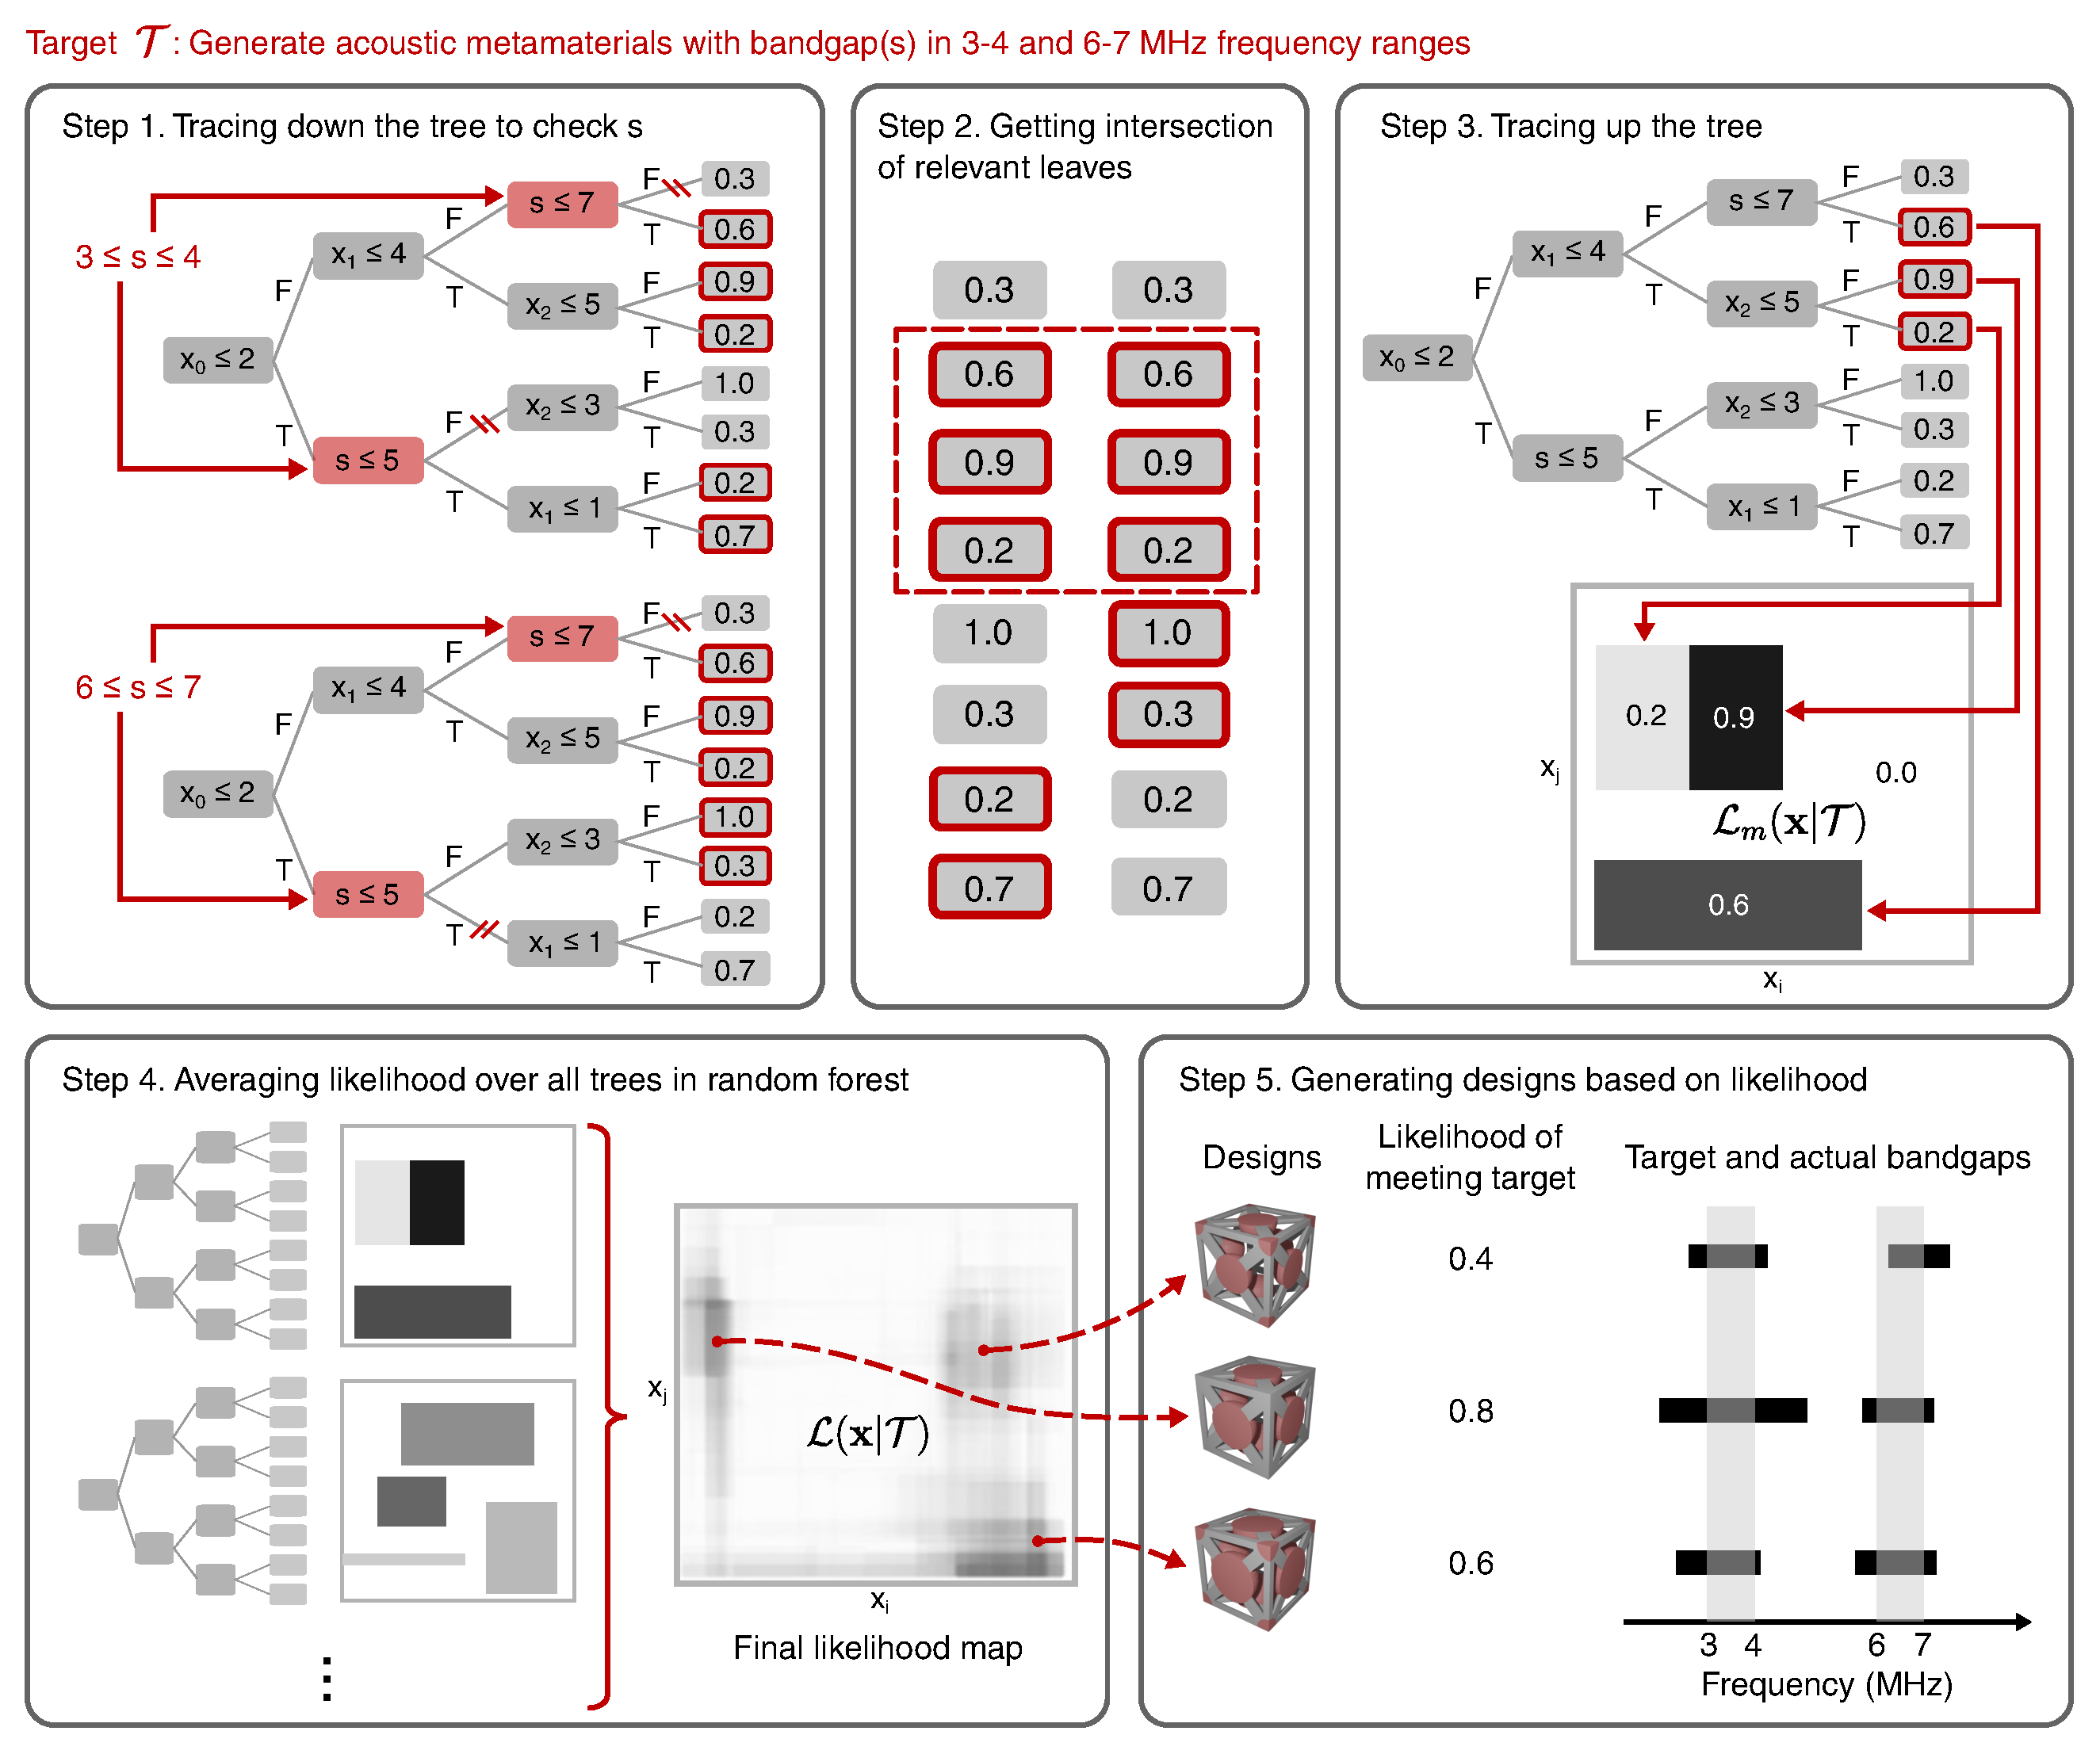
\includegraphics[width=0.9\textwidth]{fig/rigid.pdf}
\caption{The inverse design pipeline of the proposed RIGID method (using the inverse design of acoustic metamaterials as an example). Given design parameters $\mathbf{x}$ and the auxiliary variable $s$ (e.g., wave frequency), a trained random forest predicts the probability of the qualitative response $y$ (e.g., bandgap existence). Each tree in the random forest splits the joint space of $\mathbf{x}$ and $s$ into regions, each associated with a specific prediction (shown on leaf nodes). The splitting criteria are encoded in tree nodes. ``T'' means meeting a criterion and ``F'' means not meeting it. RIGID first identifies leaf nodes that are relevant to the considered range of auxiliary variable $s$ by checking splitting criteria related to $s$ and pruning tree branches that are irrelevant (Step 1). If the considered range of $s$ has multiple parts, we repeat this step for each part and take the intersection of relevant leaves (Step 2). Each relevant leaf node corresponds to a decision path indicating a region in the design space, as well as a predicted probability of target satisfaction, which is a score we assign to the corresponding design space region (Step 3). With multiple trees in a random forest, we can average the scores predicted by each tree and use the average score as our likelihood estimation (Step 4). We can then sample from the design space based on the likelihood distribution to generate new designs tailored to the target (Step 5).}
\label{fig:rigid}
\end{figure*}

Figure~\ref{fig:rigid} shows how, by probing the trained random forest, one can estimate a likelihood distribution for target satisfaction of solutions over the entire design space and sample (generate) new designs based on this likelihood distribution. Since we target qualitative (binary) behaviors at specified $s$ (e.g., a bandgap in 3-4 MHz frequency or high absorption at a wavelength of 400-500 nm), we first identify the leaf nodes (on each decision tree in the random forest) that are relevant to the $s$ in the target (Fig.~\ref{fig:rigid}, Step 1). We do this by tracing down each tree, checking only the nodes that use $s$ as the splitting feature, and pruning the branches that are irrelevant to the $s$ in the target. For example, as shown in Fig.~\ref{fig:rigid}, there are two tree nodes using $s$ as the splitting feature, with splitting criteria at $s \leq 5$ and $s \leq 7$. Given the target frequency range of $3 \leq s \leq 4$, we can remove the right branches of both nodes as these branches are only relevant to $s>5$ and $s>7$, respectively, which conflicts with the target range of $3 \leq s \leq 4$. After pruning these branches, we end up with a set of leaves relevant to the target (highlighted in Fig.~\ref{fig:rigid}, Step 1). When we have a combined target (e.g., bandgaps in both 3-4 MHz and 6-7 MHz, as shown in Fig.~\ref{fig:rigid}), we need to get the intersection of all the sets of relevant leaves and use that as the final set of relevant leaves (highlighted in Fig.~\ref{fig:rigid}, Step 2). Note that a combined target includes cases where there are multiple nonadjacent target ranges (e.g., 3-4 MHz and 6-7 MHz) or when a target range is split by a tree node (e.g., a target range of 4-6 MHz can be split by the node ``$s \leq 5$'', thus we need to consider it as the combination of two target ranges~\textemdash~4-5 MHz and 5-6 MHz). A more detailed discussion of this step is in \textit{Appendix, Sec.~\ref{sec:app_step2}}.

The next step is to trace up the tree from the $N$ relevant leaves, obtained by Step 2, to the root node (Fig.~\ref{fig:rigid}, Step 3). This will result in $N$ decision paths, along which are nodes indicating splitting criteria for design variables $\mathbf{x}$. Thus, each decision path represents a set of design variable ranges, or in other words, a region in the design space. We assign each region a score equal to the predicted probability at each corresponding leaf. This probability is learned from the training data and equals the proportion of positive data in a leaf. It indicates the tree's belief in the probability of a design $\mathbf{x}$ satisfying the target $\mathcal{T}$ if the design falls in the design space region corresponding to the leaf. Therefore, with a single decision tree $i$, we already have the map of likelihood $\mathcal{L}_m(\mathbf{x}|\mathcal{T})=\mathbb{P}_m(\mathcal{T}|\mathbf{x})$ for target satisfaction: each of the $N$ regions has a uniformly distributed likelihood equal to the predicted probability at the corresponding leaf, and the rest of the design space has a likelihood of 0 (Fig.~\ref{fig:rigid}, Step 3).

Since a single decision tree usually lacks accuracy, robustness, and a way to quantify estimation uncertainty, we still want to take advantage of the random forest as an ensemble model for inverse design. We use Steps 1-3 to derive the likelihood distribution for each of the $M$ trees in the random forest, and simply use the average of these $M$ likelihood distributions as the final likelihood for target satisfaction, $\mathcal{L}(\mathbf{x}|\mathcal{T})=\sum_m^M \mathcal{L}_m(\mathbf{x}|\mathcal{T})/M$, which is a more complex and smooth function (Fig.~\ref{fig:rigid}, Step 4). If more trees believe a design $\mathbf{x}$ has a higher likelihood of satisfying the target, then the design will have a higher likelihood $\mathcal{L}(\mathbf{x}|\mathcal{T})$. Finally, to generate new designs, we can sample from $\mathcal{L}(\mathbf{x}|\mathcal{T})$ using Markov chain Monte Carlo (MCMC) methods such as Metropolis-Hastings~\cite{hastings1970monte} (Fig.~\ref{fig:rigid}, Step 5).

Compared to prior works, RIGID provides the following unique benefits:
\begin{enumerate}
    \item It is effective on small data problems as the random forest is less susceptible to overfitting.
    \item The training is fast (in seconds of wall time) and does not require computationally-demanding hyperparameter tuning. Once the training is done, no further training or iterative optimization is required to generate designs for different targets.
    \item The model is interpretable as one can easily probe the trained model to understand its reasoning behind any decision-making.
    \item It estimates the explicit likelihood of target satisfaction for every possible solution in the design space. Given a design target of specific functional behavior, we can generate an unlimited number of solutions based on the likelihood, allowing us to explore alternative solutions that might have desired properties or functionalities beyond the ones considered as the target. 
    \item When generating design solutions, one can use a single parameter~\textemdash~the sampling threshold~\textemdash~to easily tune the trade-off between exploitation (i.e., generated designs have higher chances of satisfying the target) and exploration (i.e., generated designs cover a broader area of the design space), as we will demonstrate in Results.
\end{enumerate}



%%%%%%%%%%%%%%%%%%%%%%%%%%%%%%%%%%%%%%%%%%%%%%%
\section{Results}
\label{sec:results}

We demonstrate our RIGID method on an acoustic metamaterial design problem, an optical metasurface design problem, and two synthetic design problems. Based on a recent review article by Lee et al.~\cite{lee2023data} and other related works (e.g., \cite{bastek2022inverting}), existing single-shot inverse design methods were demonstrated on training data size ranging from $10^3$ to $10^6$ in scale. Here we show that our method can work with much smaller-scale datasets (less than 250 training samples).

For all the test problems, we used the same random forest hyperparameter settings and did not perform hyperparameter tuning. Specifically, each random forest contains 1,000 trees with a minimum of 2 samples required to split an internal node and a minimum of 1 sample required to be at a leaf node. Gini impurity~\cite{BreiFrieStonOlsh84} was used as the splitting criterion at tree nodes.
The train-test split ratio was 4:1. Since the positive/negative training data can be highly imbalanced (e.g., the frequency ranges with bandgaps are much narrower than those without), we used the Synthetic Minority Over-sampling TEchnique (SMOTE)~\cite{chawla2002smote} to over-sample the positive class. For all the case studies, the random forest training took less than 10 seconds on an Intel Core i5-9300H CPU 2.4GHz and 8GB memory.

After training, we generate new designs by sampling from the resulting likelihood distribution using Metropolis-Hastings. In practice, Metropolis-Hastings can generate identical samples, which provides no benefits for design purposes. Thus in this work, we reject the designs identical to previous ones during sampling.


\subsection{Applying RIGID to Design Acoustic Metamaterials with Target Bandgaps}
\label{sec:acoustic}
Here we consider acoustic metamaterials that can control elastic wave propagation at ultrasound (MHz) frequencies. Varying the microscale geometries of acoustic metamaterials changes the dynamic properties of a material, such as bandgaps~\cite{bayat2018wave} (i.e., forbidden frequency ranges of a material) and wave propagation direction~\cite{casadei_piezoelectric_2012}. 
These materials promise applications in waveguides~\cite{casadei_piezoelectric_2012,liu2020acoustic}, lenses~\cite{kim2021poroelastic,xie2018acoustic}, and vibration mitigation~\cite{krodel2015wide}. 
We present the braced cubic design framework (Fig. \ref{fig:acoustic}A-B) as a method to tune the size and location of bandgaps (Fig.~\ref{fig:acoustic}C). 
In particular, spherical micro-inertia are added to the center and corner of a braced cubic unit cell with strut radius $r_\text{strut}$. 
Micro-inertia placed at the center of the brace has radius $r_\text{center}$ while micro-inertia placed at the corner of the cubic unit cell has radius $r_\text{corner}$. 

\begin{figure*}[h]
\centering
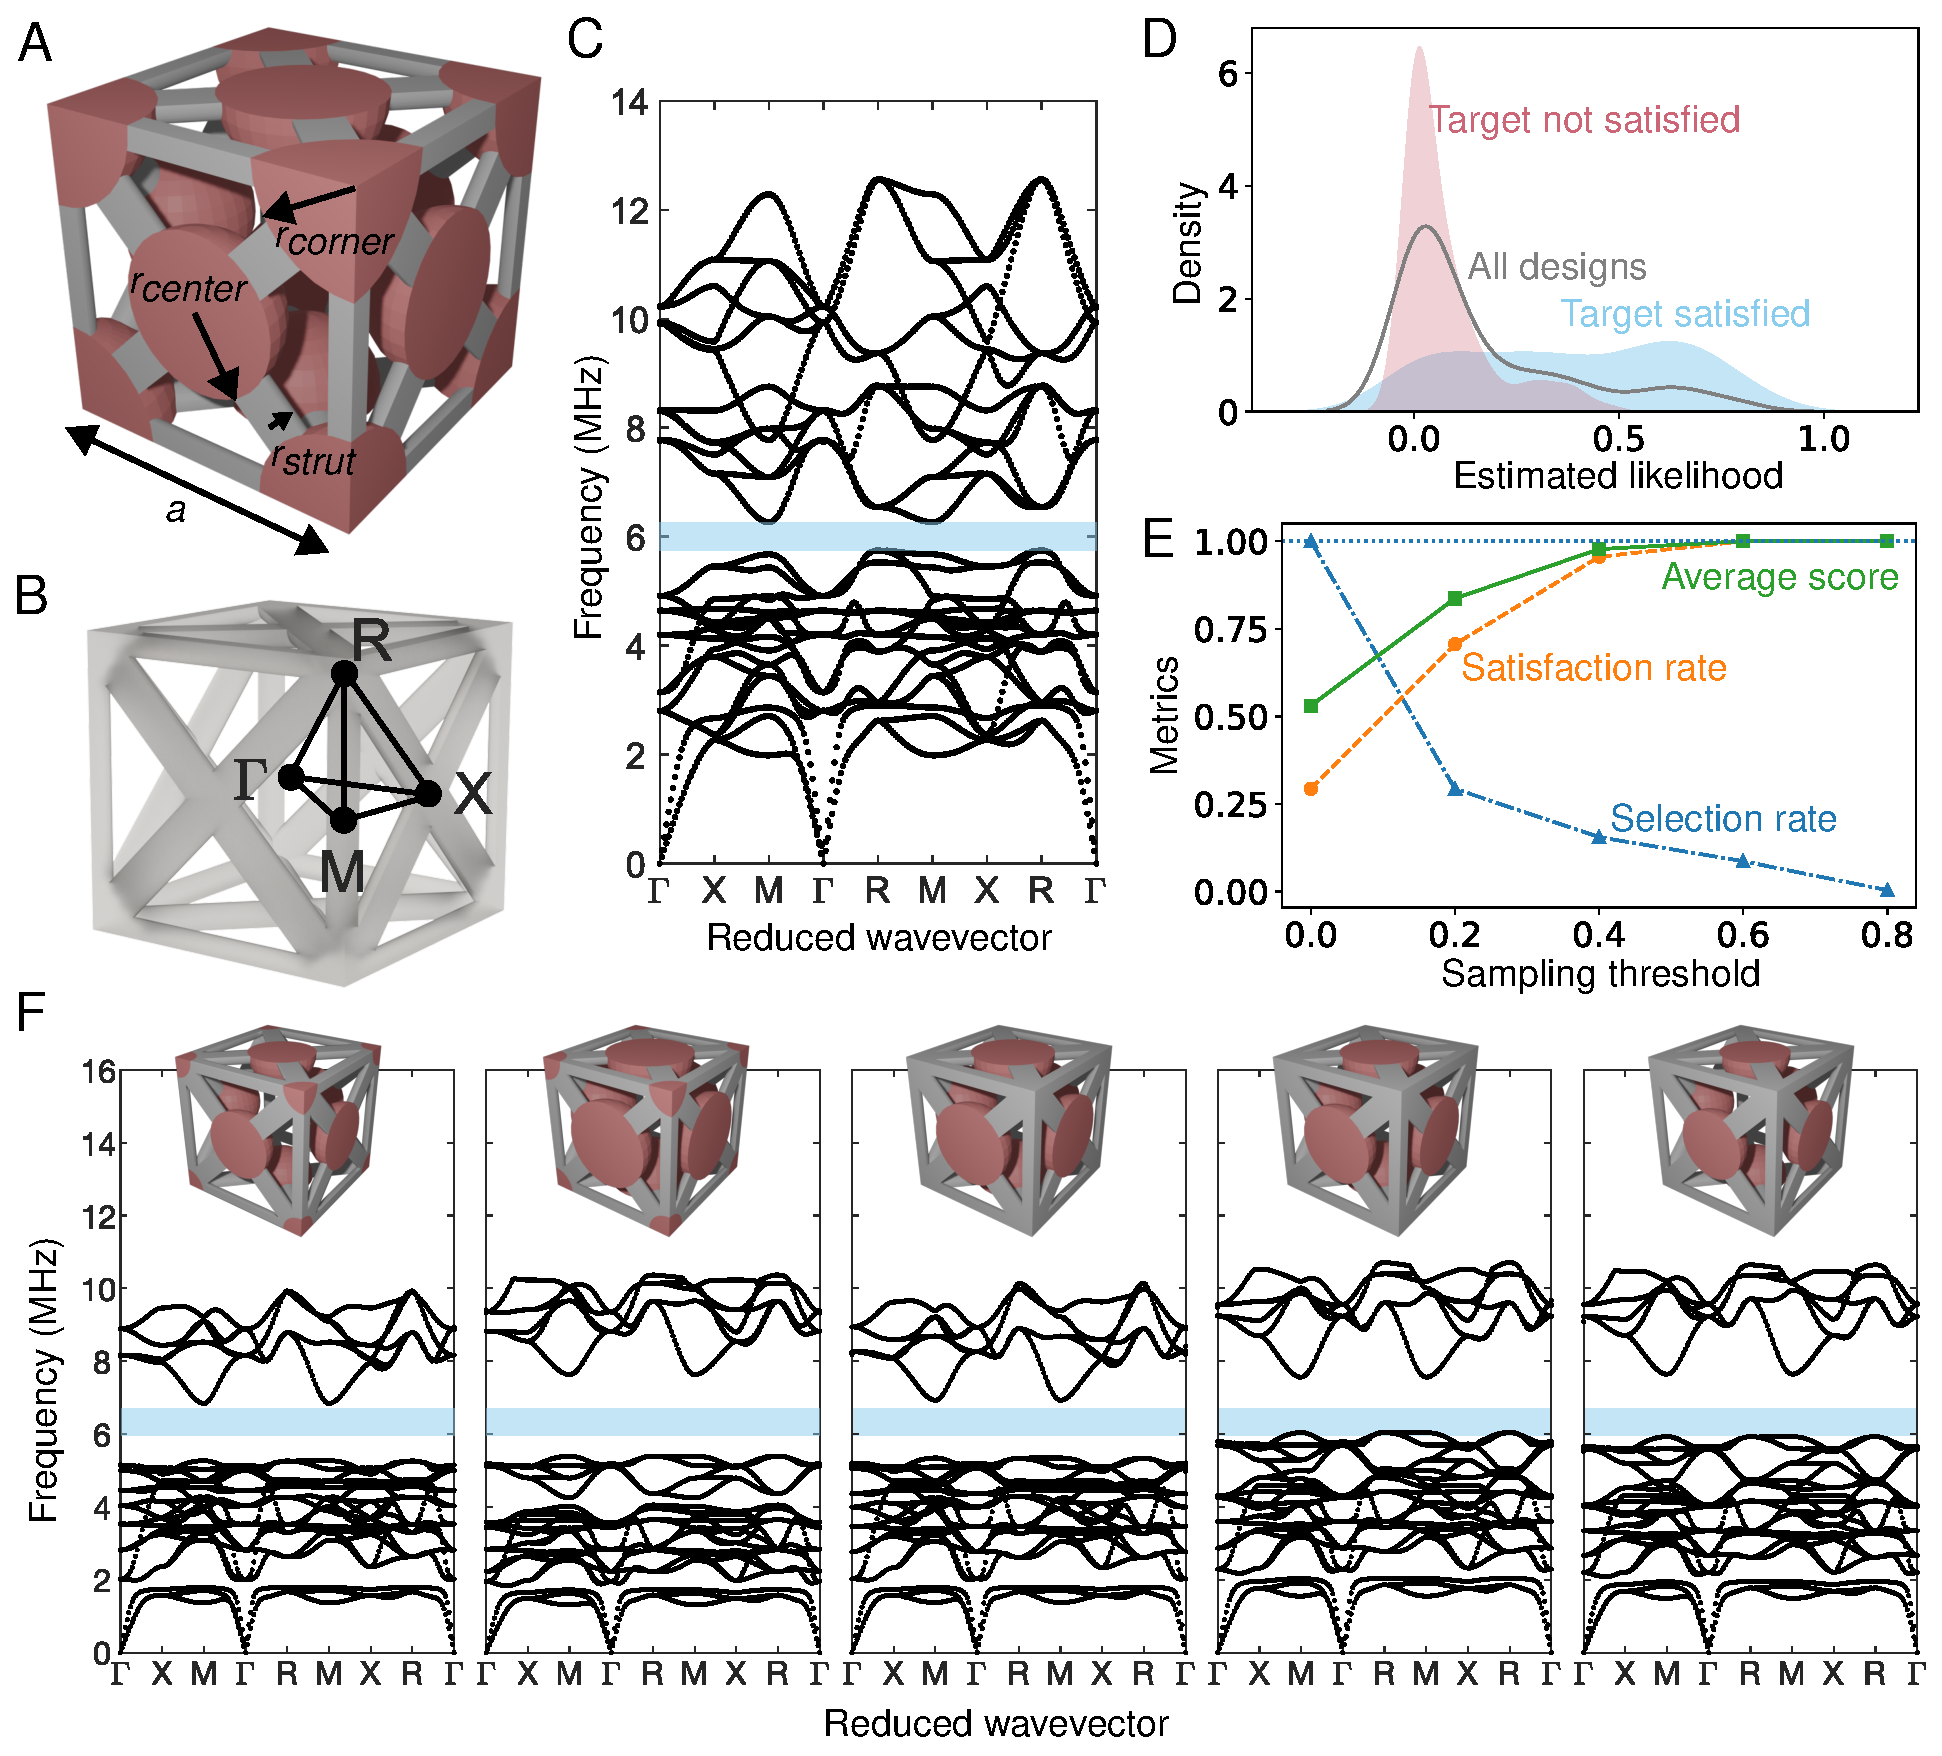
\includegraphics[width=.8\textwidth]{fig/acoustic.pdf}
\caption{Acoustic metamaterial design problem configuration and results. (A)~Design variables of center and corner mass radii ($r_\text{center}$ and $r_\text{corner}$) and strut radius ($r_\text{strut}$). (B)~High symmetry points of the cubic irreducible Brillouin zone. (C)~A sample dispersion relation and bandgap (marked by the highlighted zone). The design objective is to generate new acoustic metamaterial designs with target bandgaps. (D)~KDE of the estimated likelihood for generated designs. (E)~Validation metrics under varying sampling thresholds. (F)~Geometries and corresponding dispersion relations of five generated designs with the highest likelihood of satisfying a specified target bandgap (marked as highlighted frequency regions). Here only the fourth design fails to meet a small portion (at around 6 MHz) of the target bandgap, whereas the others meet it. Generated designs for other targets are shown in \textit{Appendix, Figs.~\ref{fig:support_acoustic_1}-\ref{fig:support_acoustic_3}}.
% The number below each geometry indicates the corresponding estimated likelihood value.
}
\label{fig:acoustic}
\end{figure*}

% ACOUSTIC METHOD (MOVE TO CORRECT SECTION) 
We randomly created 284 sets of geometric parameters $\mathbf{x} = (r_\text{strut}, r_\text{center}, r_\text{corner})$ with 4 $\leq r_\text{strut} \leq$ 6.41, 0 $\leq r_\text{center} \leq$ 20, and 0 $\leq r_\text{corner} \leq$ 20 (unit: \textmu m). The unit cell size was set at $a=60$ \textmu m. For each of these designs, we performed Bloch-wave analysis to compute its acoustic dispersion relation. 
Bandgap location and width were extracted for each design based on its dispersion relation. 

Out of the 284 sets of design variables and bandgap data, we used 227 samples as training data. We first discretized the entire frequency range into 100 intervals, and trained a random forest to predict bandgap existence $y\in\{0,1\}$ at a specific interval $s$ for a given design $\mathbf{x}$. The trained model has a test F1 score of 0.82. The resulting confusion matrix on test data is shown in \textit{Appendix, Tab.~\ref{tab:f1_acoustic}}.

To test the inverse design capability of RIGID, we randomly created 10 targets, each containing 1-2 frequency ranges in which bandgap(s) should exist. 
We generated 30 designs for each target by sampling from the resulting likelihood distribution over the design space\footnote{Note that it is possible for the likelihood to be zero everywhere in the design space when the model believes the target is unachievable. We ignore these cases as it is meaningless and impossible to sample designs from such likelihood distribution.}. Bandgaps were identified from dispersion relations computed using Bloch-wave analysis.
Figure~\ref{fig:acoustic}D shows the kernel density estimation (KDE) for the likelihood of the 300 generated designs, conditioned on their target satisfaction.
We use $\mathcal{D}$ and $\mathcal{D}_\text{feas}$ to represent the complete set of generated designs and the set of generated designs that actually satisfy the target, respectively. Then $\mathcal{D}\backslash\mathcal{D}_\text{feas}$ denotes the set of generated designs that cannot fulfill the target in reality.
In an ideal scenario, all solutions in $\mathcal{D}$ would satisfy the target, which means $\mathcal{D} = \mathcal{D}_\text{feas}$, and their density profiles should coincide. However, this ideal scenario is not possible due to limited model accuracy. Conveniently, the estimation of target satisfaction likelihood offers us an indicator of what solution is more likely to violate the target. For a reasonable model, most designs in $\mathcal{D}\backslash\mathcal{D}_\text{feas}$ should have low estimated likelihood values. Consequently, the density of $\mathcal{D}_\text{feas}$'s likelihood is a result of shifting some of $\mathcal{D}$'s density from left (low likelihood) to right (high likelihood). This expectation aligns with the observation in Fig.~\ref{fig:acoustic}D.

When sampling new designs or selecting solutions from generated designs, we can put a \textit{sampling threshold} $\tau \in (0, 1)$ on the likelihood values to filter out ``less promising'' solutions. To further examine model behavior and quantify how $\tau$ affects the inverse design outcome, we define the following metrics:
\begin{equation}
\begin{split}
\text{Selection Rate} & = \frac{|\mathcal{D}_{\phi \geq \tau}|}{|\mathcal{D}|}, \\
\text{Satisfaction Rate} & = \frac{|\mathcal{D}_{\phi \geq \tau} \cap \mathcal{D}_\text{feas}|}{|\mathcal{D}_{\phi \geq \tau}|}, \\
\text{Average Score} & = \frac{1}{|\mathcal{D}_{\phi \geq \tau}|} \sum_{i=1}^{|\mathcal{D}_{\phi \geq \tau}|} q_i, \\
\end{split}
\label{eq:metrics}
\end{equation}
where $\mathcal{D}_{\phi \geq \tau}$ is the set of generated designs with the likelihood of at least $\tau$ (i.e., the selected designs) and $q_i$ denotes the percentage overlap between the target and the actual behavior of selected designs.
The satisfaction rate evaluates how many selected designs satisfy the target based on a binary criterion (i.e., whether or not a design satisfies the complete target), whereas the average score provides a soft measure where partial satisfaction is also counted. The average score is lower-bounded by the satisfaction rate.

As shown in Fig.~\ref{fig:acoustic}E, the selection rate decreases when $\tau$ increases since more solutions are filtered out. On the other hand, both the satisfaction rate and the average score increase with $\tau$, which indicates a high correlation between the estimated likelihood of a solution and its probability of actually achieving the target. As $\tau$ reaches 0.6, the satisfaction rate and the average score reach 1, indicating that all generated designs satisfy their targets. When sampling or selecting new solutions, we can use the sample threshold $\tau$ to tune the trade-off between exploitation and exploration~\textemdash~a low $\tau$ favors exploration as sampled solutions will cover a larger area of the design space, while a high $\tau$ favors exploitation as sampled solutions will have a higher chance of satisfying the target.

Figure~\ref{fig:acoustic}F visualizes the geometries and dispersion relations of designs generated based on a randomly created bandgap target. Only the top five designs with the highest likelihood values are shown.
% Although these designs exhibit different geometries and dispersion relations, most of them satisfy the target. 
In this example, our method generates geometrically different designs that have a high probability of achieving target bandgaps, each yielding a slightly different dispersion relation. This is promising in design applications requiring other material properties, such as dynamic wave velocity or quasi-static stiffness, in which the user can select from a menu of designs with the same target bandgap but other varying properties. Generated designs based on the other nine bandgap targets can be found in \textit{Appendix, Figs.~\ref{fig:support_acoustic_1}-\ref{fig:support_acoustic_3}}.






\subsection{Applying RIGID to Design Optical Metasurfaces with Target High-Absorbance Wavelengths}
\label{sec:optical}

Optical metasurfaces are artificially engineered systems that can support exotic light propagation building on subwavelength inclusions~\cite{pendry2000negative, yu2011light, kildishev2013planar, cui2014coding, bukhari2019metasurfaces, hu2021review}. Among a diverse array of devices, metamaterial absorbers~\cite{landy2008perfect, liu2010infrared, hao2010high, watts2012metamaterial, cui2014plasmonic, liu2017experimental, lee2018complete} have been intensely studied for medical imaging, sensing, and wireless communications.

In this case study, we consider four types of cross-sections ($c \in \{1,2,3,4\}$) chosen from the literature (Fig.~\ref{fig:optical}B). It is assumed that a 3D geometric instance is composed of a stack of three layers of prismatic unit cells, each of which is vertically extruded and stacked (Fig.~\ref{fig:optical}A). The geometries constructed in this way can be regarded as an instantiation of multilayered metasurfaces~\cite{zhou2018multilayer, li2018wideband, marino2021harmonic, malek2022multifunctional, zhang2023high}, which offer richer design freedom than the single-layer counterpart. The height of each layer ($h_l, l=1, 2, 3$) is allowed to continuously vary between 50 and 150 nm. Herein we do not consider parametric variations of a given type of unit cell cross-section; yet those can be trivially incorporated in the proposed design framework if necessary.

\begin{figure*}[h]
\centering
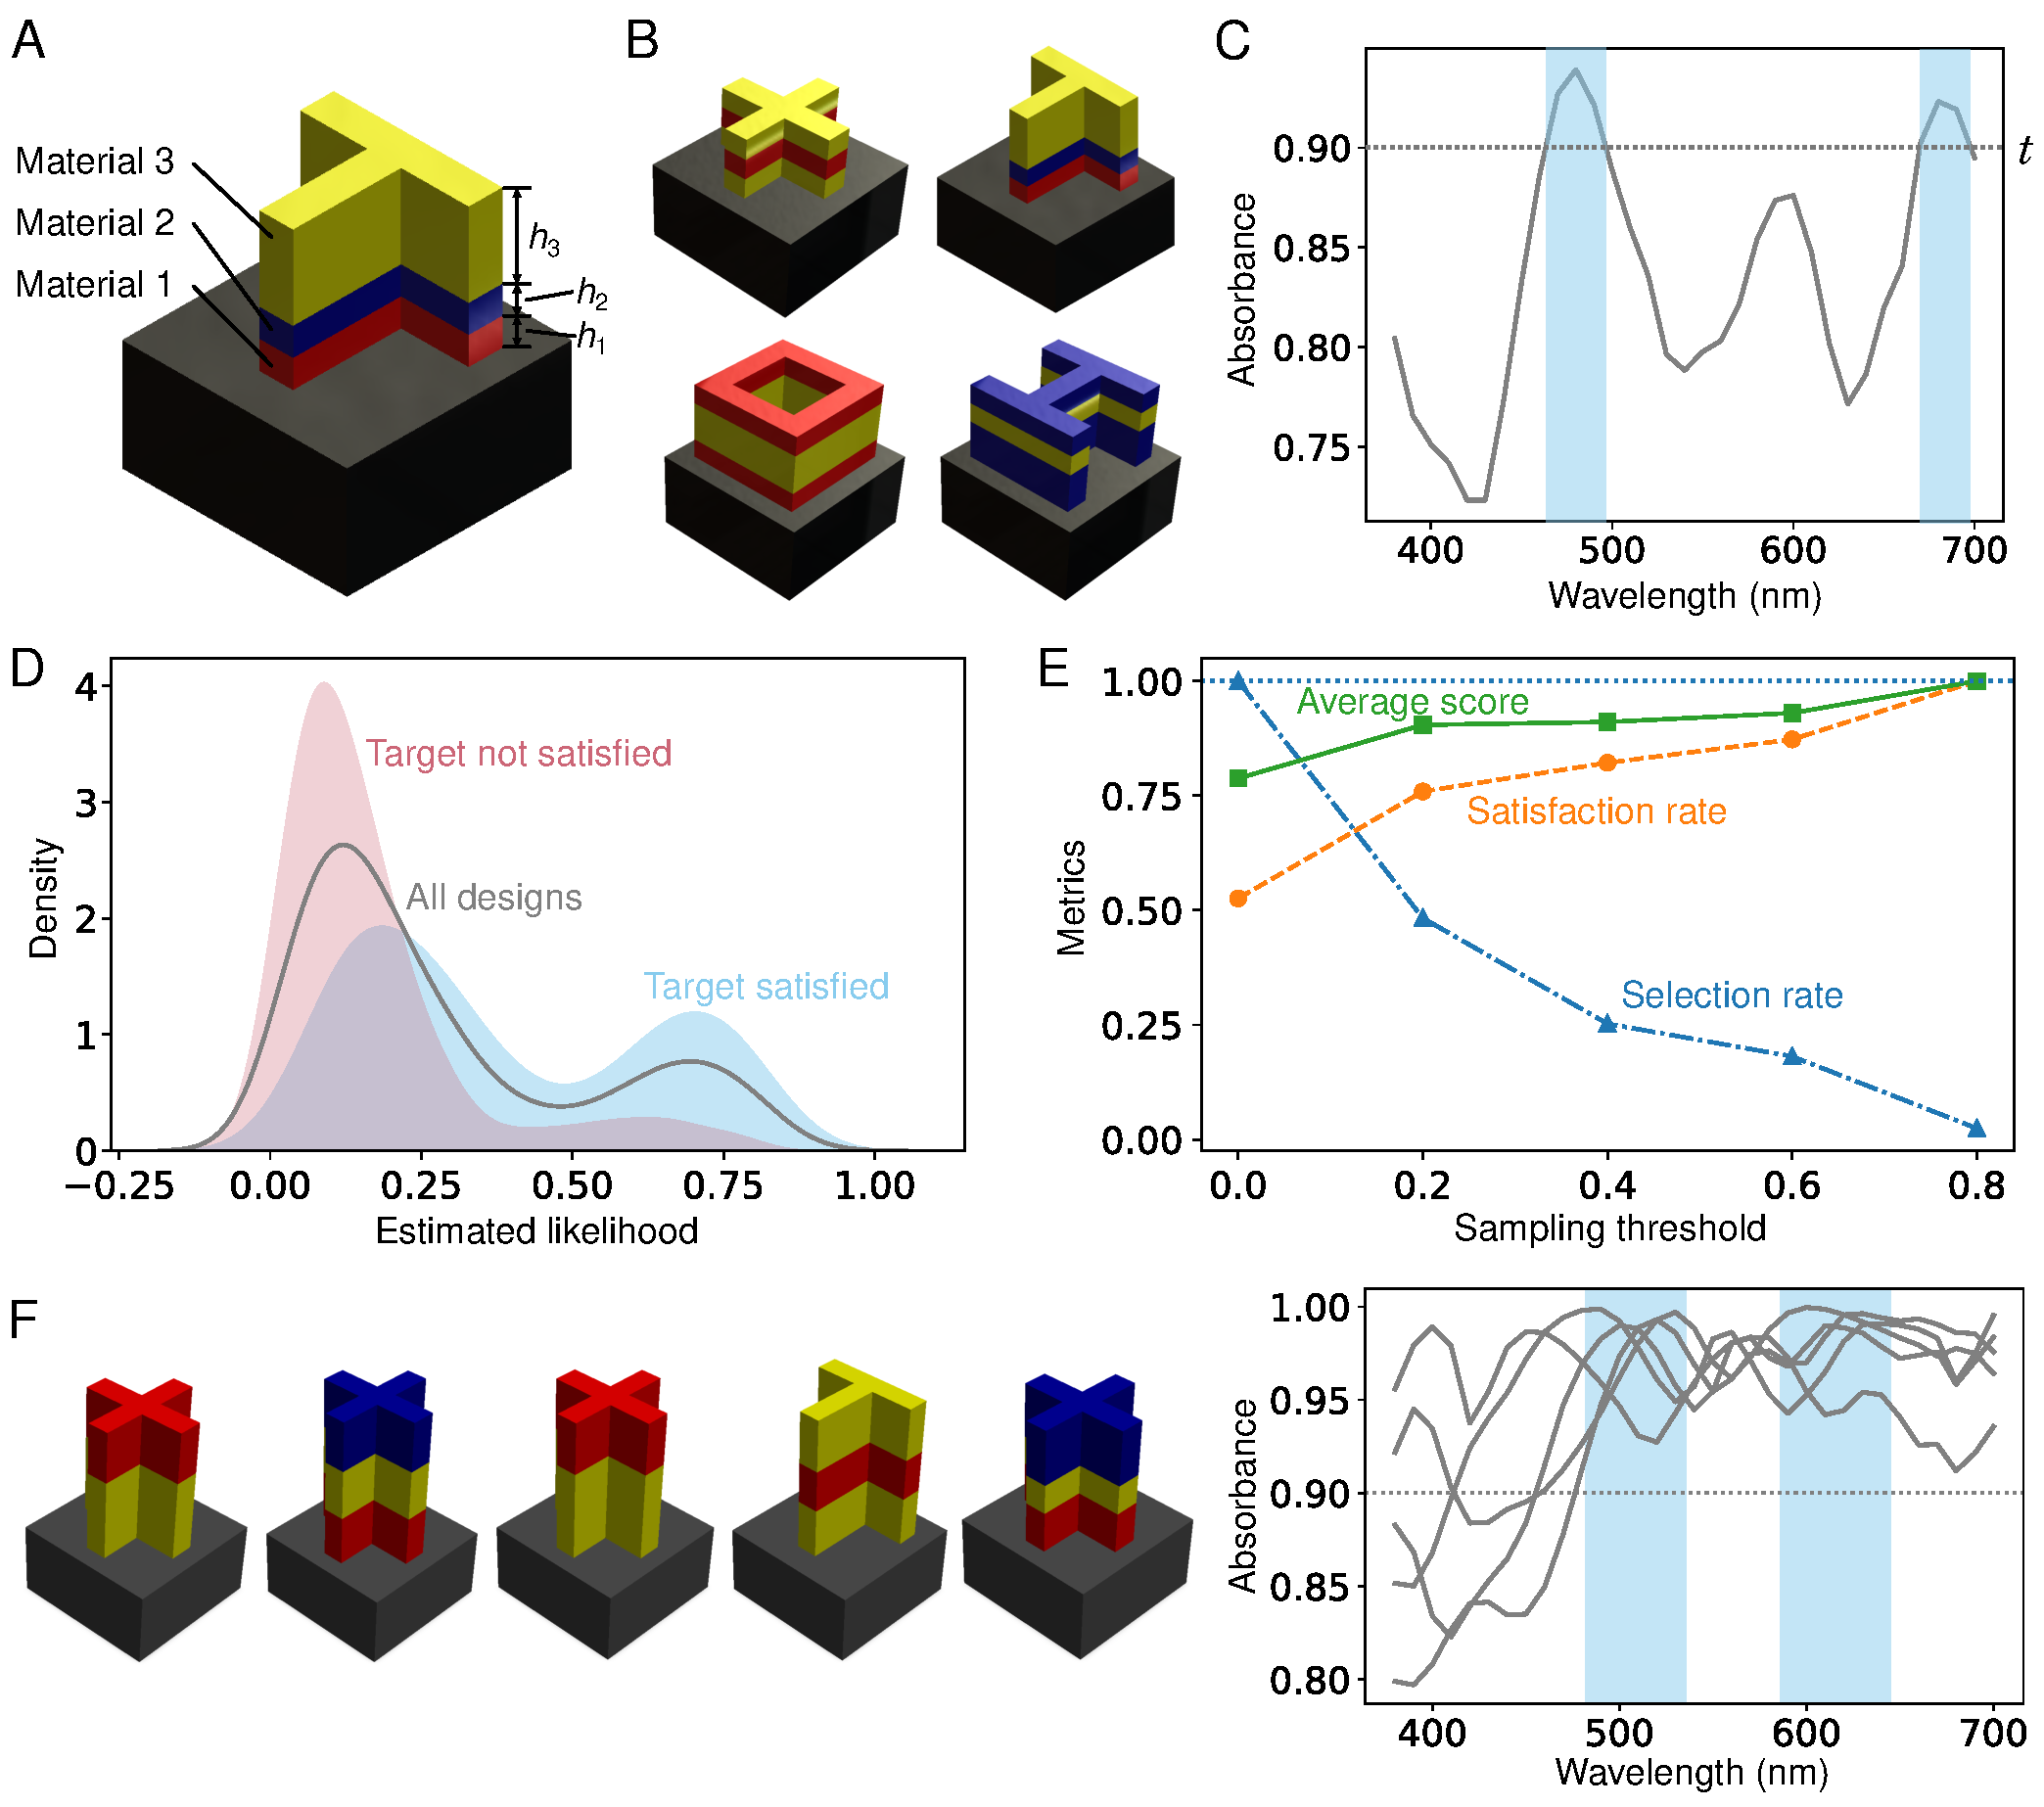
\includegraphics[width=0.8\textwidth]{fig/optical.pdf}
\caption{Optical metasurface design problem configuration and results. (A-B)~Design variables (materials, layer heights, and cross-section geometry types). (C)~A sample absorbance spectrum and the wavelength intervals (highlighted wavelength regions) corresponding to absorbance above the threshold $t$. The design objective is to generate new optical metasurface designs that exhibit higher absorbance than a threshold $t$ at the user-defined wavelength interval(s). (D)~KDE of the estimated likelihood for generated designs. (E)~Validation metrics under varying sampling thresholds. (F)~Designs (geometries and material selections) and corresponding absorbance spectra of five generated metasurfaces with the highest likelihood of satisfying specified target high-absorbance regions (marked as highlighted wavelength regions). Here all five designs satisfy the target. Generated designs for other targets are shown in \textit{Appendix, Figs.~\ref{fig:support_optical_1}-\ref{fig:support_optical_2}}.
% The number below each design indicates the corresponding estimated likelihood value.
}
\label{fig:optical}
\end{figure*}

We also design the material of each layer ($m_l, l=1, 2, 3$). Three dielectric materials of interest, each of which is assigned to a different color in Fig.~\ref{fig:optical}A, are Ti (red), Si (blue), and Ge (yellow). In general, a dielectric material is characterized through a complex refractive index $ \Tilde{n} \in \mathbb{C}$ defined as $\Tilde{n} = n + j k$, where $j=\sqrt{-1}$ is the imaginary unit, $n\in\mathbb{R}$ involves the speed at which the light propagates through the material, and $k\in\mathbb{R}$ is the extinction coefficient that dictates the energy loss due to the material.
Within the frequency regime of interest, those exhibit nonlinear dispersion; both the real and imaginary terms in general are a non-analytic function of excitation wavelength $s$, i.e., $n(s)$ and $k(s)$. In addition, the impact of the same material choice on the spectral response $A(s)$ varies depending on the layer location at which the material is placed. Thus the highlight of this case study is the combinatorial nature of design, whose spectral responses are affected by the joint contributions of geometry and material.

Based on the above configuration, we randomly sampled 258 sets of design variables $\mathbf{x} = (c, h_1, h_2, h_3, m_1, m_2, m_3)$ and computed their corresponding absorbance spectra using wave analysis. We set $t=0.9$ as the absorbance threshold, so that ``high'' absorbance means the absorbance $A(s)$ is no less than 0.9. We trained a random forest on 206 training data (i.e., 80\% of the 258 designs and corresponding absorbance spectra) to predict whether ``high'' absorbance is presented (i.e., the binary indicator $y=1$) at a wavelength $s$ for a given design $\mathbf{x}$. The trained random forest has a test F1 score of 0.83. The confusion matrix on test data is shown in \textit{Appendix, Tab.~\ref{tab:f1_optical}}.

Note that this problem involves inverse design with both continuous and categorical variables, which common optimization and generative modeling-based inverse design cannot handle well without special treatment~\cite{zhang2020bayesian,ma2020vaem,xu2018synthesizing}. On the other hand, our random forest-based method can naturally address such mixed-variable problems without any issues.

Similar to the acoustic metamaterial design problem, we use 10 randomly created targets to evaluate the inverse design performance of RIGID, except that here a target is represented as the wavelength range(s) within which absorbance should be at least 0.9. We generated 100 designs for each target by sampling from the estimated likelihood distribution. Among the 1,000 generated solutions, we successfully conducted wave analysis for 911 designs and obtained their absorbance spectra. Figure~\ref{fig:optical}D shows the KDE for the likelihood of these 911 designs, conditioned on their target satisfaction. The densities share similar behavior as in the acoustic problem (Fig.~\ref{fig:acoustic}D)~\textemdash unsatisfied/infeasible designs $\mathcal{D}\backslash\mathcal{D}_\text{feas}$ are concentrated at low likelihood regions, which causes the likelihood density of satisfied/feasible designs $\mathcal{D}_\text{feas}$ to be a result of shifting some of $\mathcal{D}$'s density from left (low likelihood) to right (high likelihood). The sampling threshold and metrics relation shown in Fig.~\ref{fig:optical}E also follow the same trend as in the acoustic problem (Fig.~\ref{fig:acoustic}E), which again demonstrates a strong positive correlation between the estimated likelihood and the probability of generated designs actually achieving their targets.

Figure~\ref{fig:optical}F shows generated optical metasurface designs with the top five likelihood estimations for a randomly created target. While the materials, cross-section geometries, and layer heights of generated designs can be different, all the designs satisfy the target (Fig.~\ref{fig:optical}F, right panel). To further enhance the diversity of final solutions, we can use sampling strategies such as the one proposed in Ref.~\cite{chan2021metaset,lee2023t} to identify a subset (of generated solutions) that simultaneously exhibits high likelihood and high diversity. Generated designs based on the other nine targets can be found in \textit{Appendix, Figs.~\ref{fig:support_optical_1}-\ref{fig:support_optical_2}}.




\subsection{Synthetic Design Problems for Rapid Validation and Visualization}
\label{sec:synthetic}

While the above metamaterial design problems represent practical use cases, the validation study is time-consuming due to the expensive computation of metamaterials' responses such as dispersion relations and absorbance spectra. To allow fast validation of the proposed method and easier inspection of the estimated likelihood in the design space, we create two synthetic case studies. Both problems have 2-dimensional ``design spaces'' that allow easy visualization.

\begin{figure*}[h]
\centering
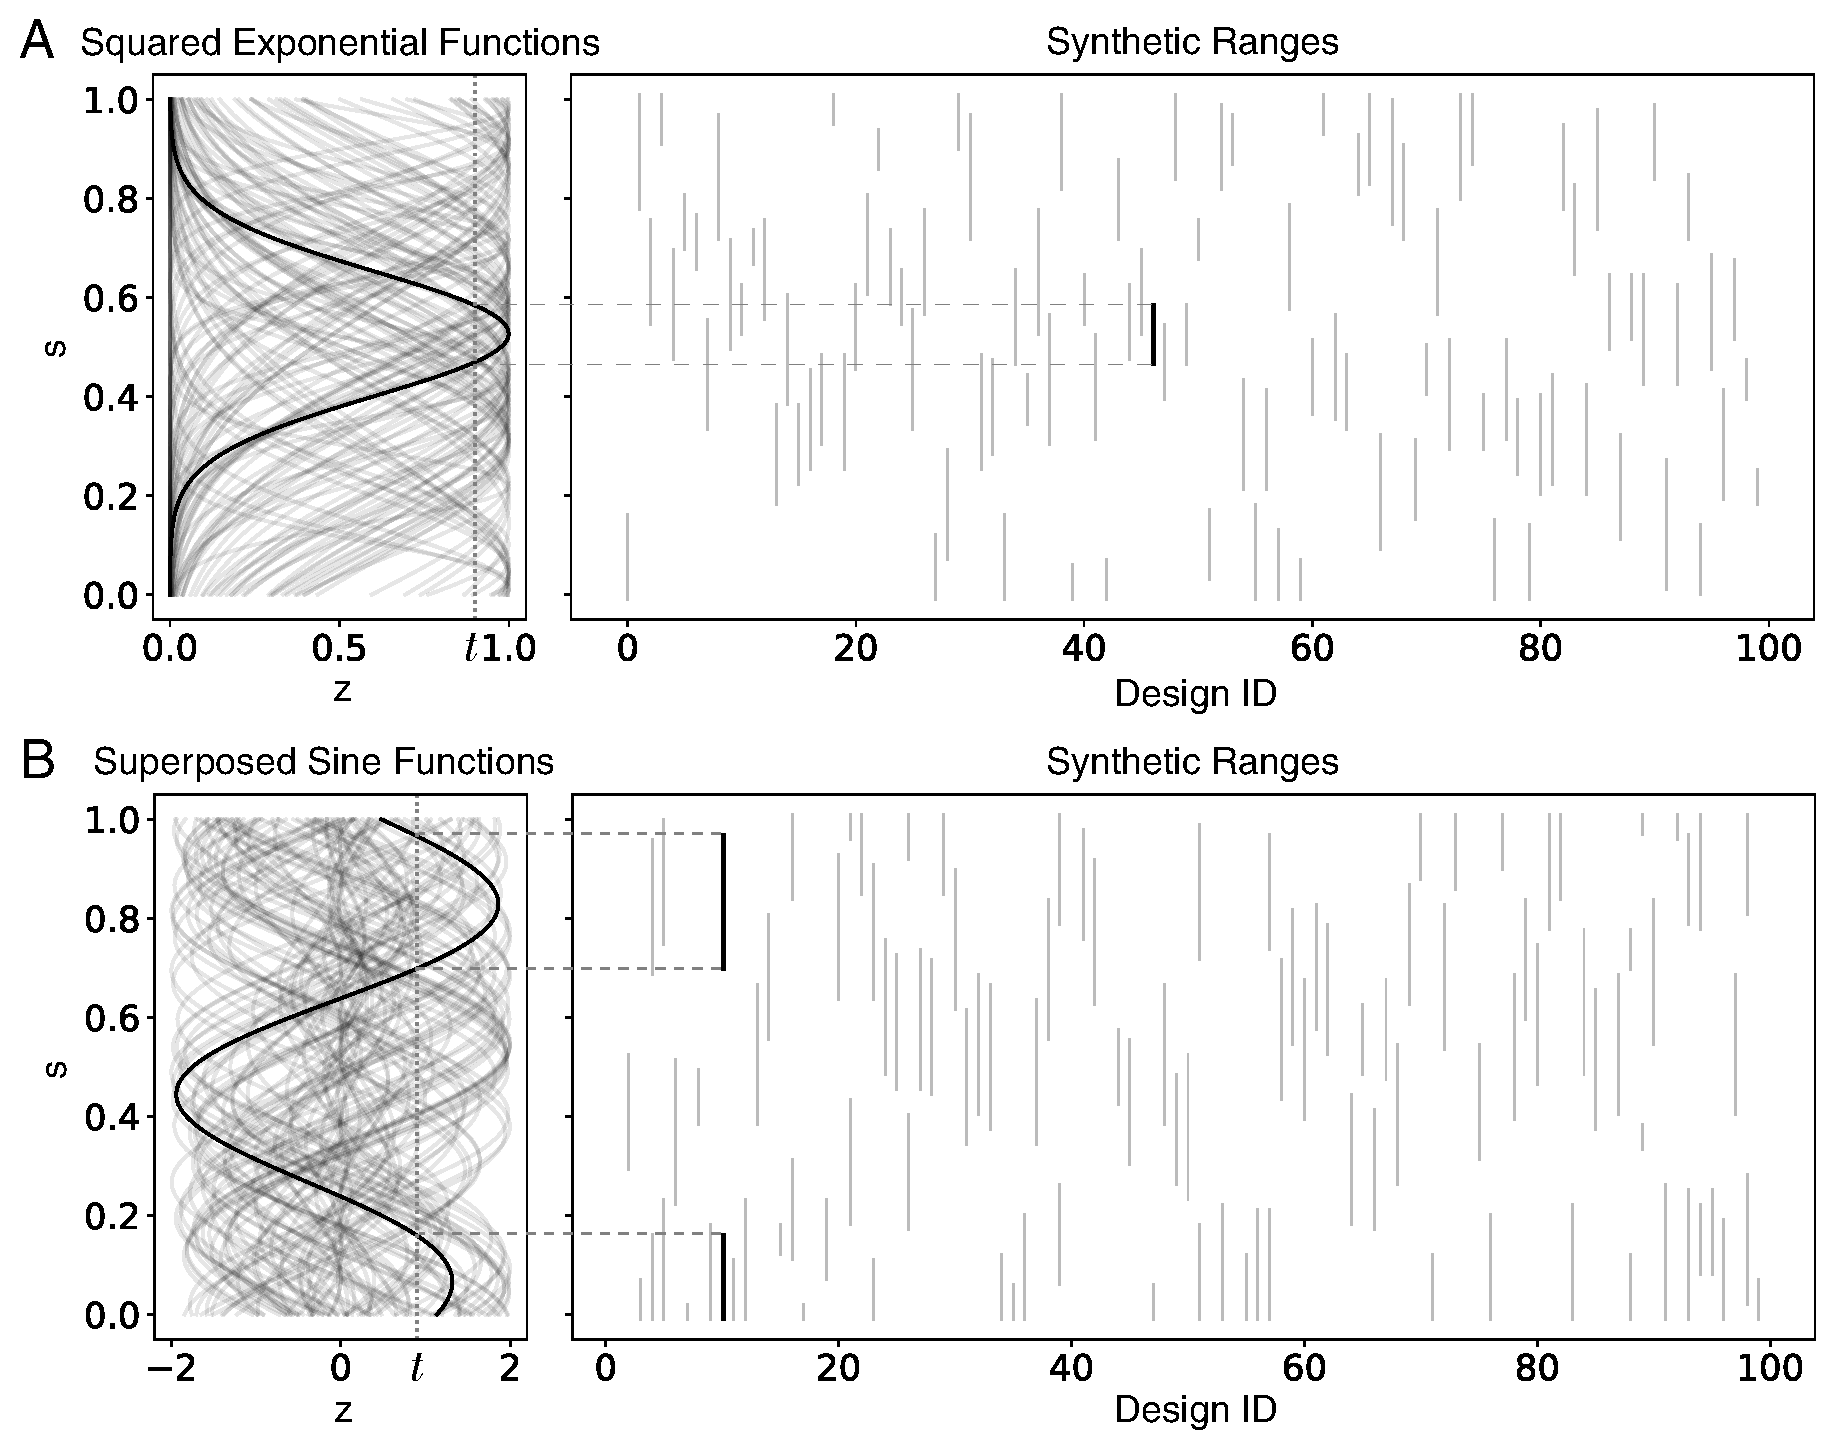
\includegraphics[width=0.8\textwidth]{fig/synthetic_data.pdf}
\caption{Synthetic data creation for (A) the SqExp problem and (B) the SupSin problem. For each problem, the left panel shows 100 functions with randomly sampled parameters $a$ and $b$. We treat $a$ and $b$ as synthetic design variables, and the corresponding functions as quantitative responses (e.g., absorbance spectra of optical metasurfaces). The right panel shows qualitative responses (e.g., high-absorbance wavelength ranges or bandgaps) are simulated by synthetic ranges, derived by thresholding the 100 functions (Equations~\ref{eq:test_func_sqexp} and \ref{eq:test_func_sin} with threshold $t$=0.9).}
\label{fig:synthetic_data}
\end{figure*}

\paragraph{SqExp Problem} To construct the first synthetic problem, we used a \textit{squared exponential function} with tunable parameters $a$ and $b$ to mimic the quantitative functional response of metamaterials. The qualitative response (e.g., ``high'' or ``low'' energy absorption at a wavelength) is defined as: 
\begin{equation}
I(a,b; s) =
    \begin{cases}
      0, & \text{if $z = \exp\left(-{\left(\frac{s-a}{0.3b+0.1}\right)^2}\right) < t$} \\
      1, & \text{otherwise}
    \end{cases},
\label{eq:test_func_sqexp}
\end{equation}
where $z$ represents quantitative response and $t$ is a threshold that converts $z$ into a qualitative response $I(a,b; s)$. Specifically, $I(a,b; s) = 1$ can mean the existence of a bandgap or high absorbance at a frequency $s$. Then $\{s|I(a,b; s) = 1\}$ represents a range of $s$ that mimics our design targets, such as the bandgap or the frequency range of high absorbance. By varying $a$ and $b$, we can produce different synthetic responses and ranges. Therefore, we can use $a$ and $b$ as synthetic design variables. There is a clear relation between these design variables and the range that Eq.~\ref{eq:test_func_sqexp} creates~\textemdash~$a$ and $b$ control the center location and the width of the range, respectively.

In this design problem, we sampled 100 sets of $a$ and $b$ uniformly at random. We set $t$ as 0.9. Based on Eq.~\ref{eq:test_func_sqexp}, we obtained the corresponding responses (Fig.~\ref{fig:synthetic_data}A). These sets of $a$, $b$, and responses constitute a dataset for training and testing our model. 

\paragraph{SupSin Problem} Another synthetic design problem was constructed by replacing
the squared exponential function in the SqExp problem with a \textit{superposed sine function}. Given synthetic design variables $a$ and $b$, we can produce qualitative responses using the following equation:
\begin{equation}
I(a,b; s) =
    \begin{cases}
      0, & \text{if $z = \sin\left(2\pi(s+a)\right) + \sin\left(3\pi(s+b)\right) < t$} \\
      1, & \text{otherwise}
    \end{cases}.
\label{eq:test_func_sin}
\end{equation}
Same as in the SqExp problem, we set $t=0.9$ and created a dataset with 100 sets of synthetic design variables and corresponding ranges derived from synthetic responses (Fig.~\ref{fig:synthetic_data}B). 
Unlike the squared exponential function, the superposed sine function can be multimodal, which means it can result in multiple synthetic ranges to mimic, for example, multiple bandgaps. The bandgap locations are controlled by $a$ and $b$.


% \begin{SCfigure*}
% \centering
% 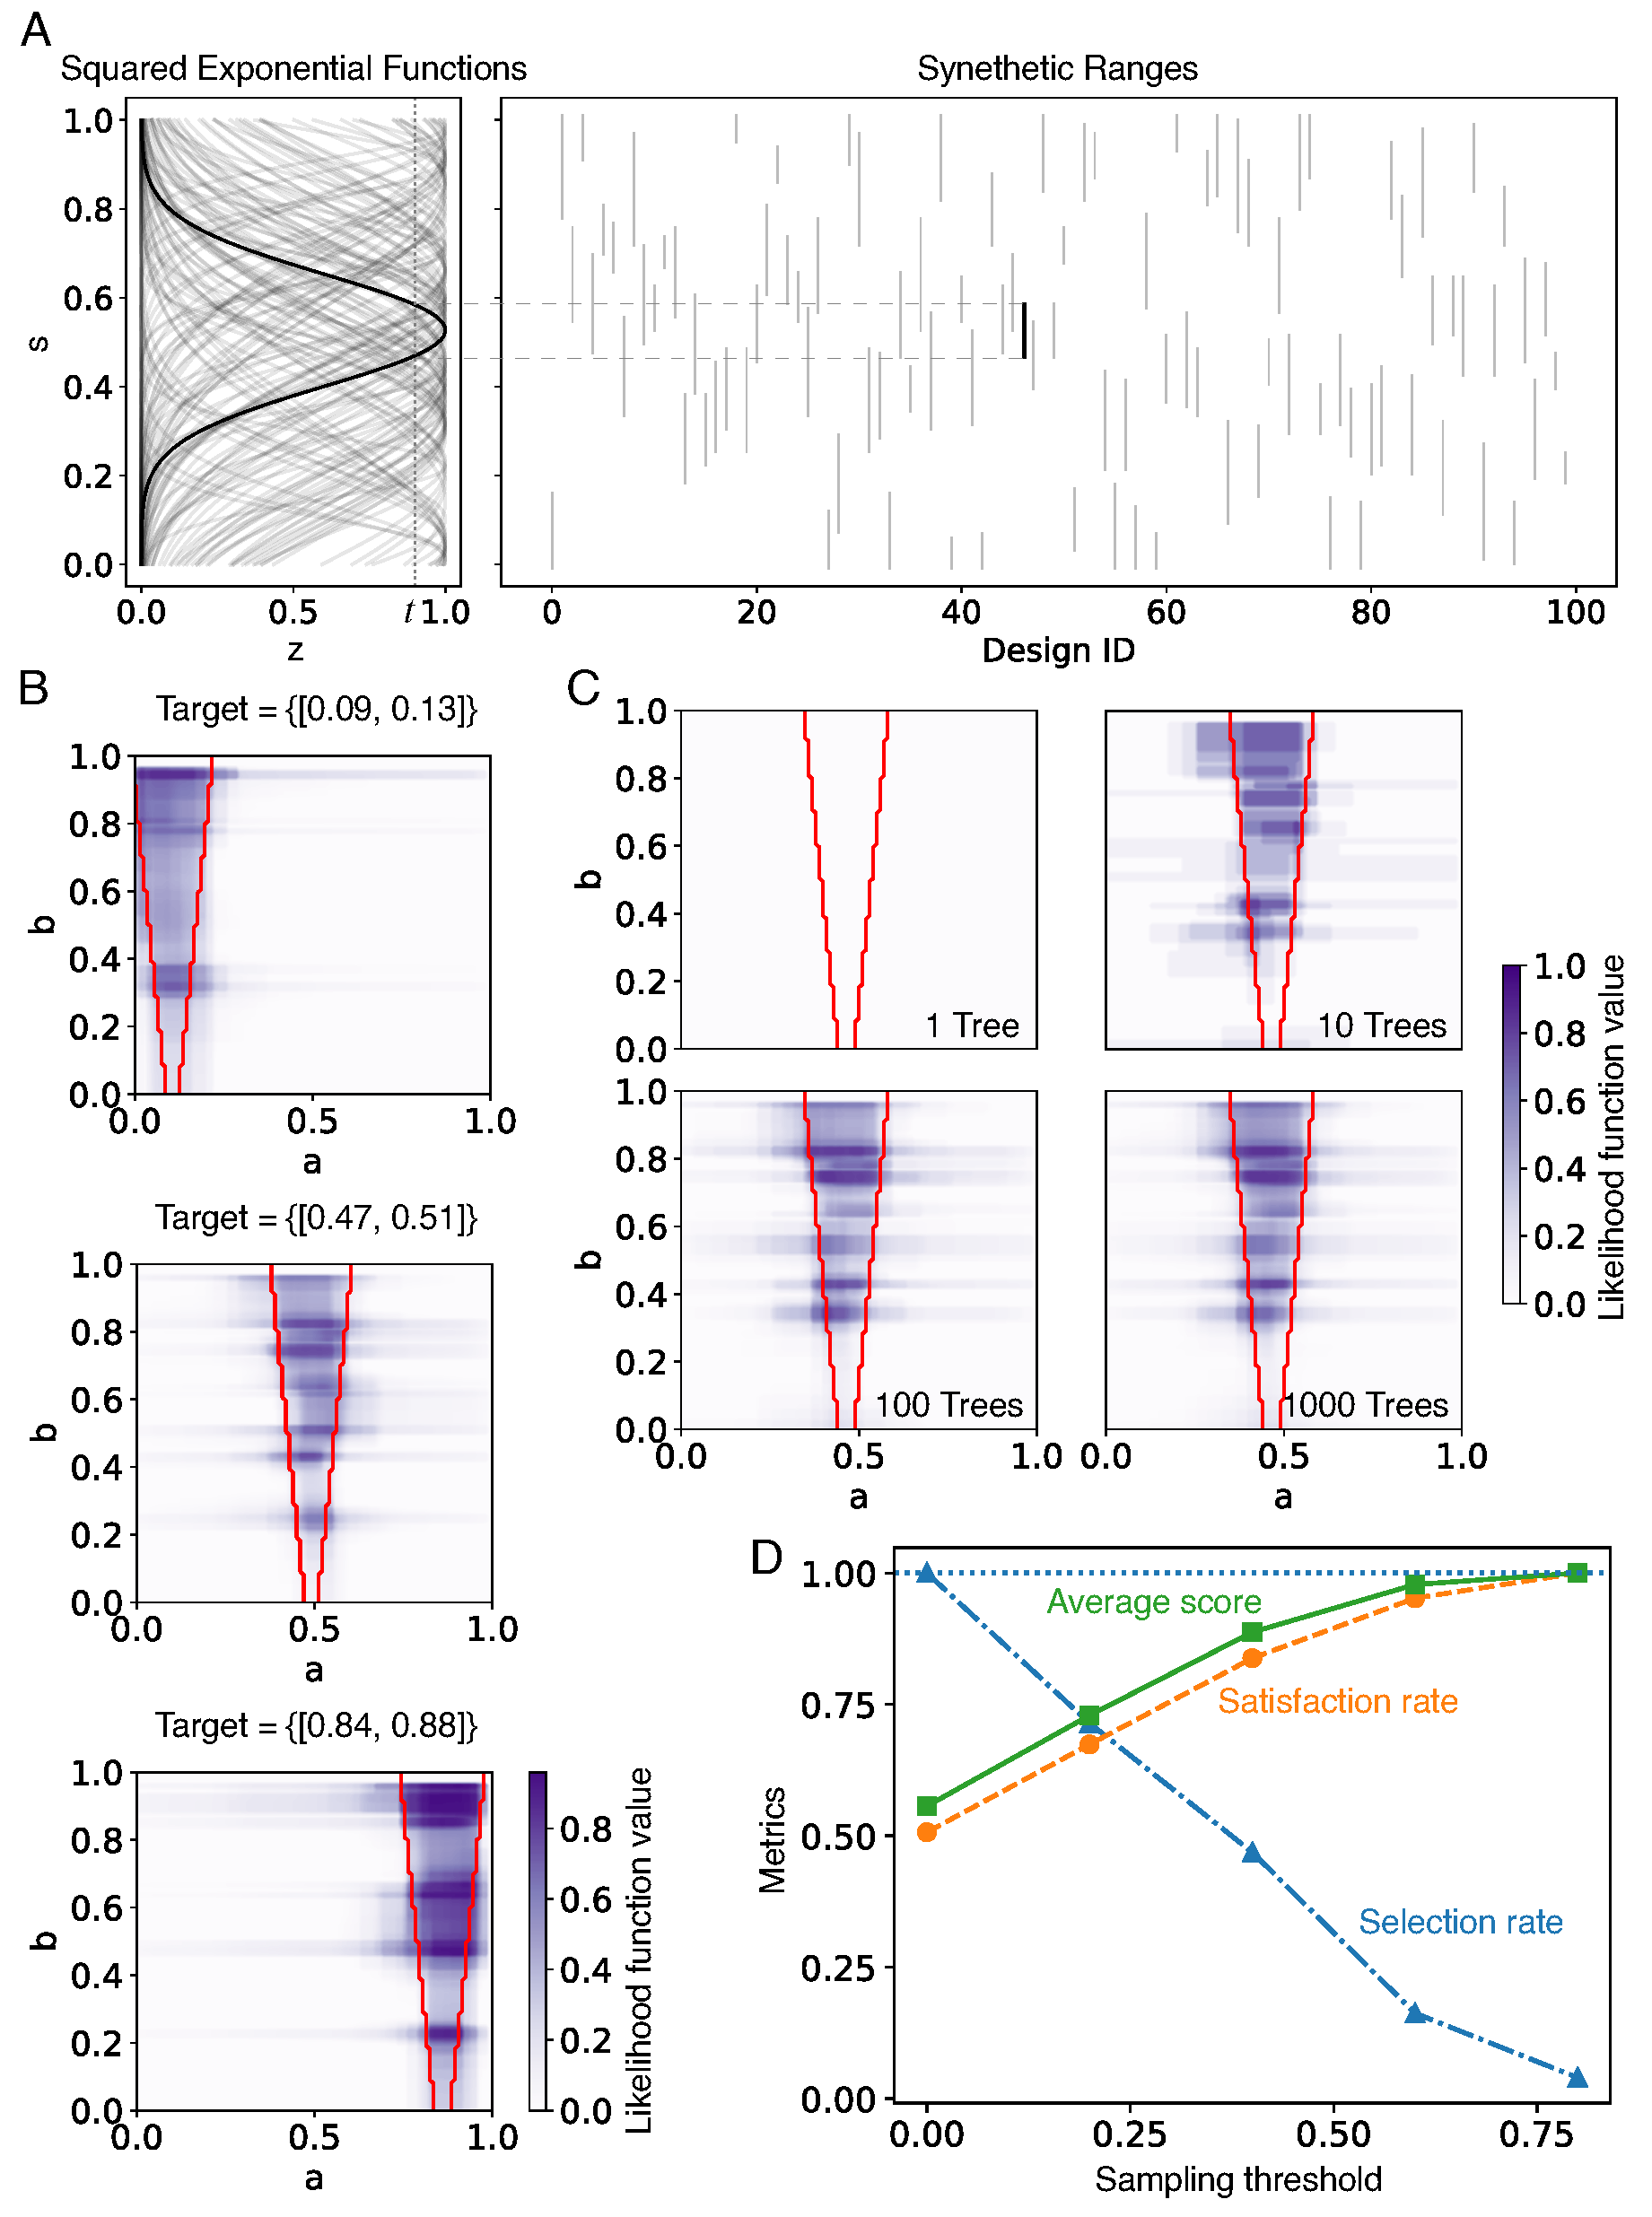
\includegraphics[width=0.7\textwidth]{fig/synthetic_sqexp.pdf}
% \caption{Synthetic data creation and method validation in the SqExp problem. (A)~100 squared exponential functions with randomly sampled parameters $a$ and $b$. We treat $a$ and $b$ as synthetic design variables. Qualitative responses (e.g., bandgaps and high-absorbance wavelength ranges) are simulated by synthetic ranges, derived by thresholding the 100 functions (Eq.~\ref{eq:test_func_sqexp} with threshold $t$=0.9). (B)~Likelihood function values for randomly created design targets. Red lines show boundaries of actual feasible regions associated with the targets. (C)~Likelihood function values estimated by random forests with varying numbers of decision trees. The design target is set as $\{[0.45, 0.48]\}$. (D)~Validation metrics for inverse design generation.}
% \label{fig:synthetic_sqexp}
% \end{SCfigure*}

% \begin{SCfigure*}
% \centering
% \includegraphics[width=0.7\textwidth]{fig/synthetic_supsin.pdf}
% \caption{Synthetic data creation and method validation in the SupSin problem. (A)~100 squared exponential functions with randomly sampled parameters $a$ and $b$. We treat $a$ and $b$ as synthetic design variables. Qualitative responses (e.g., bandgaps and high-absorbance wavelength ranges) are simulated by synthetic ranges, derived by thresholding the 100 functions (Eq.~\ref{eq:test_func_sin} with threshold $t$=0.9). (B)~Likelihood function values for randomly created design targets. Red lines show boundaries of actual feasible regions associated with the targets. (C)~Likelihood function values estimated by random forests with varying numbers of decision trees. The design target is set as $\{[0.63, 0.68], [0.69, 0.71]\}$. (D)~Validation metrics for inverse design generation.}
% \label{fig:synthetic_supsin}
% \end{SCfigure*}

For each synthetic example, we split the data into 80 training data and 20 test data, and trained a random forest, with the same hyperparameter settings as the other problems, to predict the binary indicators $I(a,b; s)$. The F1 scores are 0.85 and 0.86 for the SqExp and the SupSin problems, respectively. The resulting confusion matrices are shown in \textit{Appendix, Tables~\ref{tab:f1_test_func_sqexp}-\ref{tab:f1_test_func_sin}}. We evaluated the inverse design performance with the trained models.

\begin{figure*}
\centering
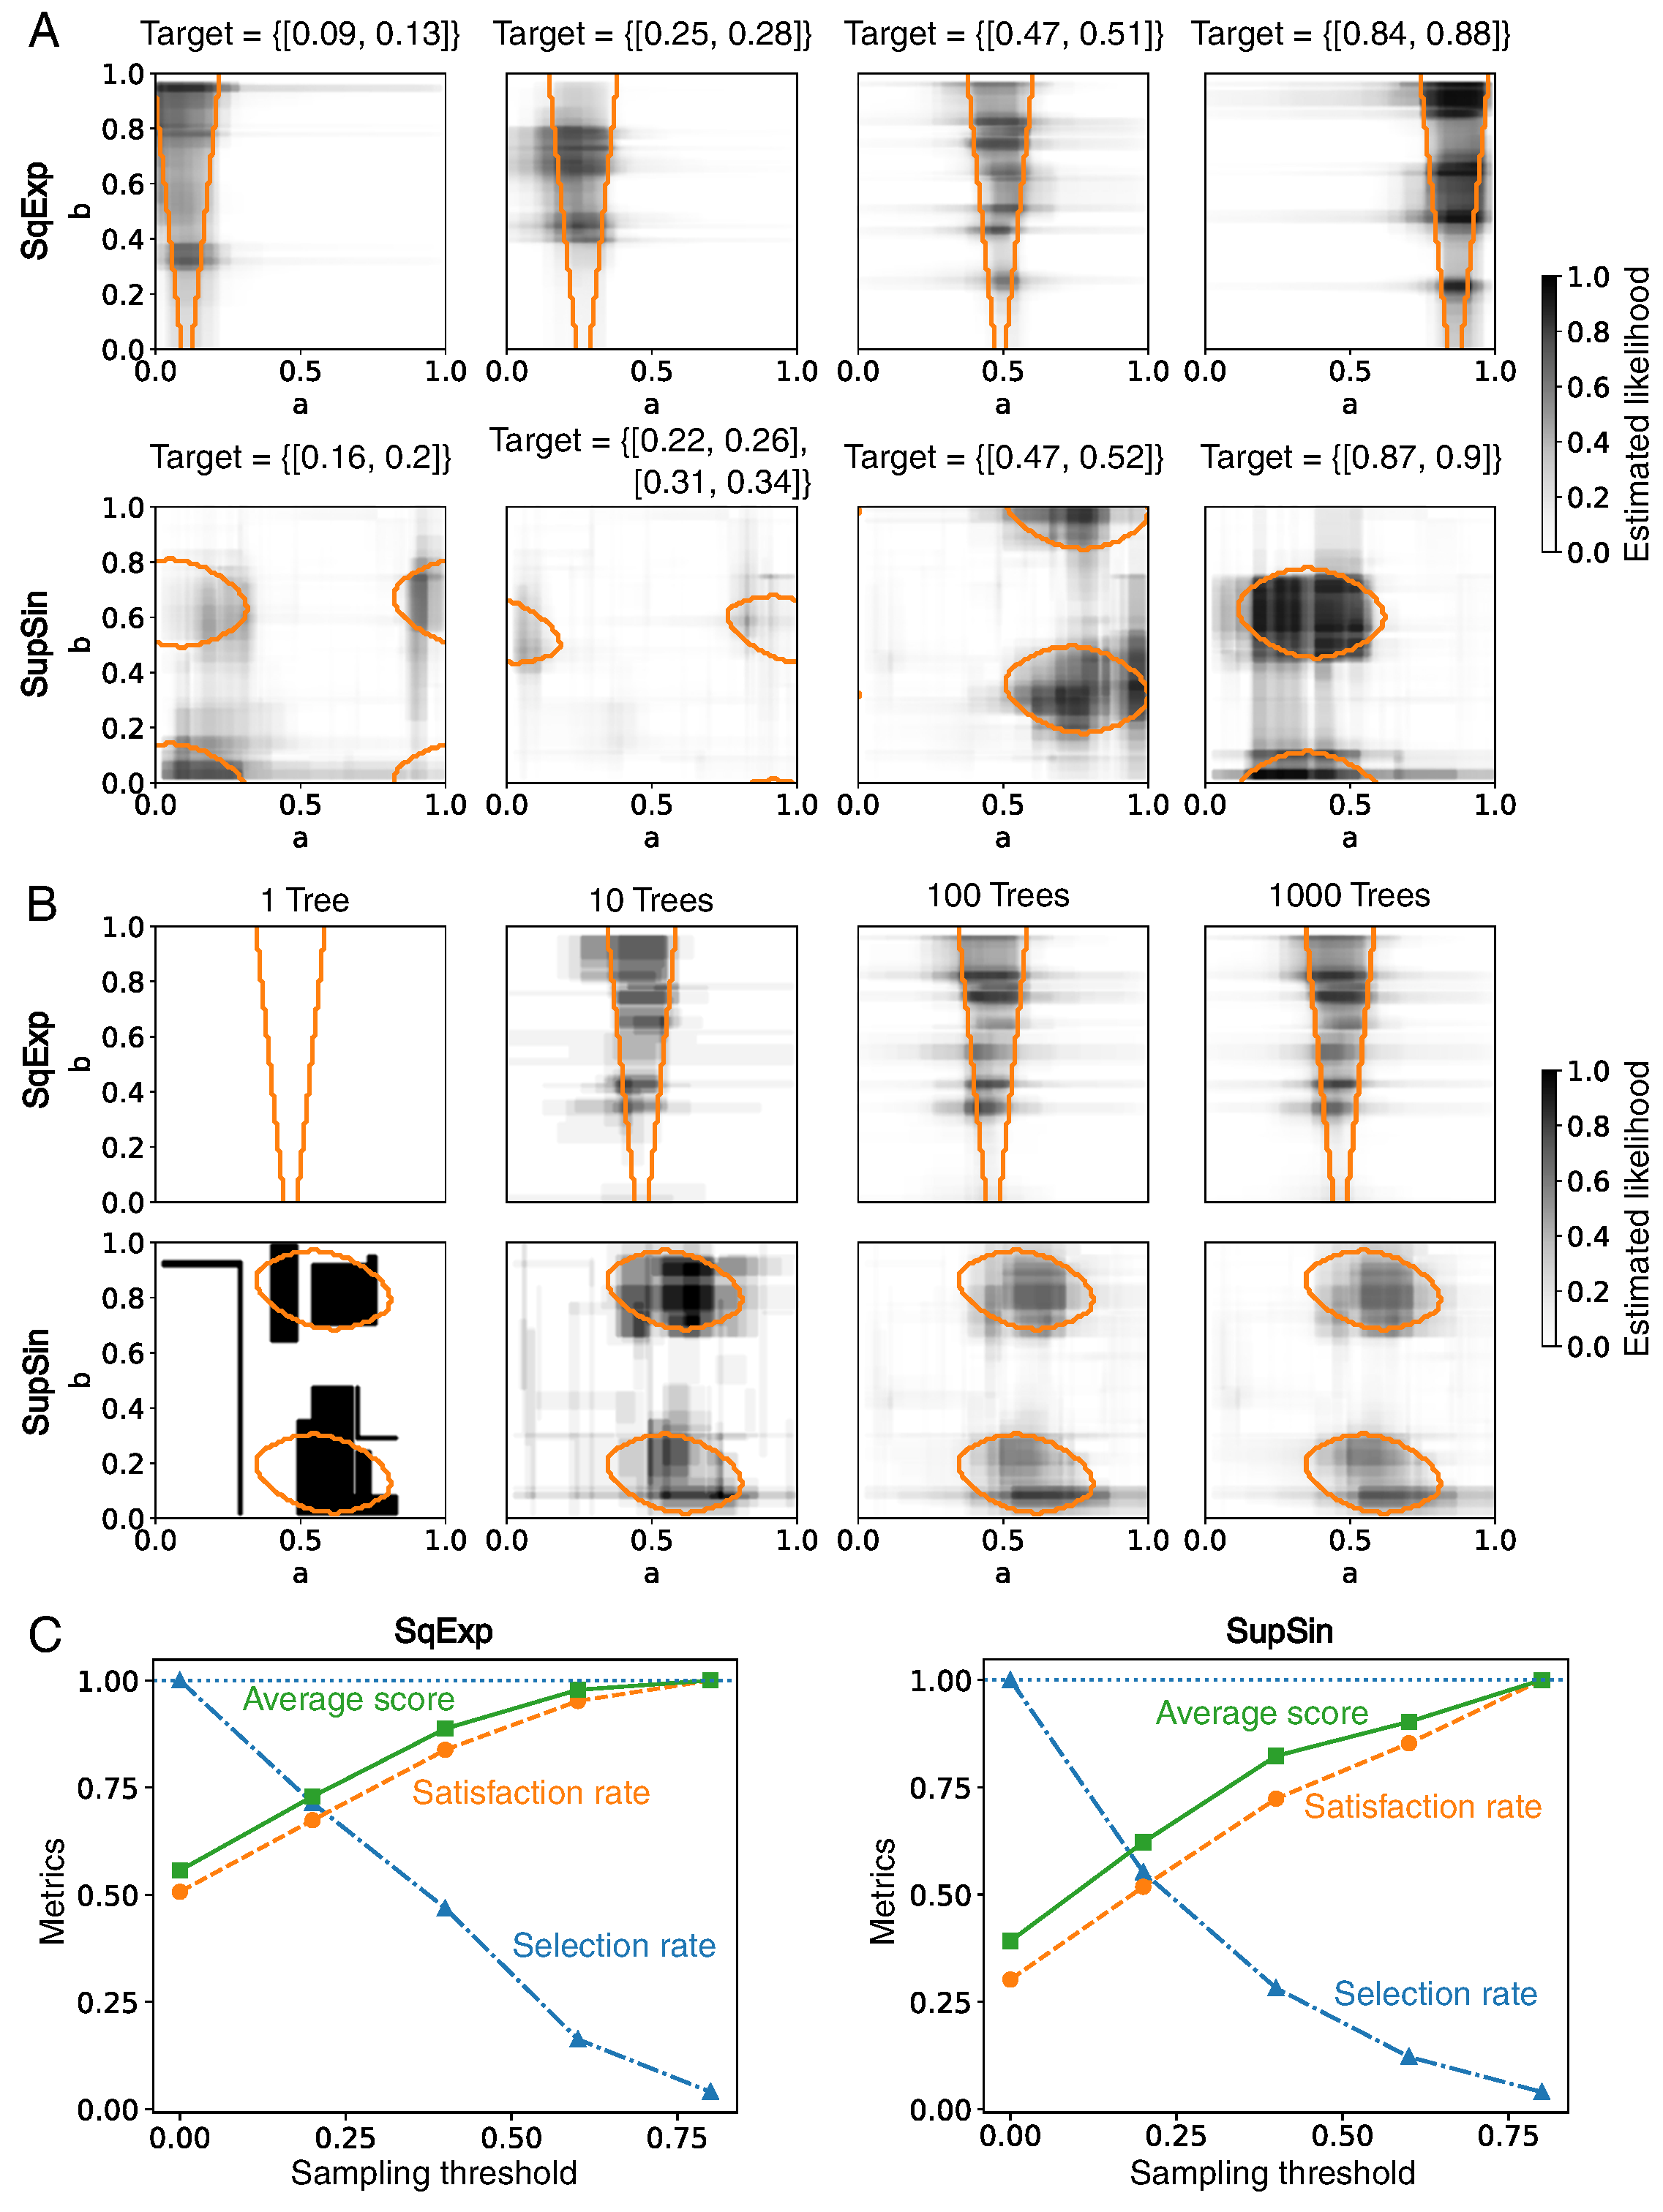
\includegraphics[width=0.8\textwidth]{fig/synthetic_results.pdf}
\caption{Visualization of estimated likelihood and validation metrics for synthetic problems. (A)~Likelihood function values for randomly created design targets. Orange lines show boundaries of actual feasible regions associated with the targets. (B)~Likelihood function values estimated by random forests with varying numbers of decision trees. The design target is set as $\{[0.45, 0.48]\}$ for the SqExp problem and $\{[0.63, 0.68], [0.69, 0.71]\}$ for the SupSin problem. (C)~Validation metrics for inverse design generation.}
\label{fig:synthetic_results}
\end{figure*}

Due to the fast evaluation of Equations~\ref{eq:test_func_sqexp} and \ref{eq:test_func_sin}, we can exhaust all the possible solutions in the design space to obtain the ground-truth feasible region(s) for a target. Figure~\ref{fig:synthetic_results}A shows the estimated likelihood values and the ground-truth feasible regions under randomly created targets. In general, high-likelihood regions match actual feasible regions well, which further demonstrates the effectiveness of RIGID. We can also observe that feasible regions in the SqExp and the SupSin problems follow distinct patterns. In the SqExp problem, $a$ and $b$ control the center location and the width of the output range, respectively. Therefore, the position of the feasible region along the $a$-axis moves with the location of the target range, while the feasible region gradually shrinks as $b$ decreases since the decrease of $b$ (i.e., output range width) causes the choice of $a$ (i.e., output range center location) to be more restricted to fit the target range. In the SupSin problem, there might be multiple bandgaps appearing at the peaks of the superposed sine function in Eq.~\ref{eq:test_func_sin}. Design variables $a$ and $b$ control bandgap locations by translating each sine function. Due to the sine function's periodicity, we can obtain multiple feasible regions along both $a$- and $b$-axes.
Figure~\ref{fig:synthetic_results}A shows that the likelihood estimation by RIGID successfully captured the above-mentioned patterns of feasible regions.

Figure~\ref{fig:synthetic_results}B demonstrates how the estimated likelihood varies when increasing the number of trees in a random forest. With a single decision tree, the estimated likelihood function is almost a binary function and highly inaccurate. The likelihood in the SqExp case is even zero everywhere, which makes it impossible to sample designs based on the likelihood. As the number of trees increases, the likelihood function becomes smoother and eventually converges.

Besides these qualitative visual inspections, we also calculated the metrics proposed in Eq.~\ref{eq:metrics}, as shown in Fig.~\ref{fig:synthetic_results}C. For each of the two synthetic problems, these metrics were computed on 500 designs generated by giving five random target ranges. Again, the satisfaction rate and the average score increase with the sampling threshold, indicating a strong correlation between the sampling threshold and the probability of generated designs actually achieving their targets. In both problems, all the selected designs satisfy their targets (i.e., the satisfaction rates and average scores reach 1) when the sampling threshold reaches 0.8.





%%%%%%%%%%%%%%%%%%%%%%%%%%%%%%%%%%%%%%%%%%%%%%%
\section{Summary and Outlook}
\label{sec:conclusion}

We proposed RIGID, a single-shot inverse design method that generates metamaterials to satisfy qualitative behaviors of functional responses. Such qualitative behaviors are important design targets in many applications such as tailoring bandgaps of acoustic metamaterials for wave-guiding, focusing, and vibration mitigation, or tailoring the absorption level of optical metasurfaces at certain wavelengths for medical sensing, imaging, and communication applications. Unlike most existing inverse design methods that require training an inverse model to map targets to designs, the RIGID method takes advantage of the random forest's interpretability and derives the likelihood of target satisfaction by probing the trained forward model. Incorporated with MCMC, one can sample a desired number of new designs based on the estimated likelihood. Therefore, RIGID functions as a generative model that can capture the conditional distribution of satisfying designs given a target, or in other words, the one-to-many mapping from the target to satisfying designs. Using both real-world and synthetic design problems, we demonstrated that RIGID is efficient and effective on datasets with training sample sizes smaller than 250. Thus, RIGID is particularly useful when data collection is expensive, as in many cases where high-fidelity simulation or experimental data are needed. We used both qualitative and quantitative approaches to validate the proposed method. The quantitative results revealed a strong correlation between the estimated likelihood of a solution and its probability of actually achieving the target, which demonstrated the effectiveness of the likelihood estimation. Due to the fast evaluation of output responses and the transparency of ground-truth solutions, the proposed synthetic problems can be used for future benchmarking studies of metamaterial design problems.

While we address qualitative design targets in this study, the idea of using random forest-based models for inverse design has the potential to generalize to quantitative targets. Such problems can be, for example, generating optical metasurface designs with specific optical spectra~\cite{liu2018generative, ma2019probabilistic}, generating functional materials with target nonlinear constitutive relations~\cite{lew2023single,vlassis2023denoising}, or generating programmable metamaterials with prescribed functional responses~\cite{li2022digital,lin2023mechanical}. It is also straightforward to adjust the target to achieve multifunctionality (e.g., negative/positive Poisson’s ratio under low/high compression rate~\cite{bossart2021oligomodal}).

Although this study only demonstrates the RIGID method on parametric design (i.e., designs are represented by geometric and/or material parameters), the method also applies to shape or topological design problems where the shape or topology of designs can vary without being restricted to a limited number of geometric parameters~\cite{liu2018generative,jiang2019free,ma2019probabilistic,wen2020robust,an2021multifunctional}. In those cases, as valid designs only lie on a lower-dimensional manifold of the design space, the likelihood of target satisfaction will be zero almost everywhere in the original design space. Thus before applying RIGID, we need to obtain a latent representation that compactly captures the manifold of valid designs~\cite{wang2020deep,chen2023gan}, and use the latent representation as design variables for inverse design.



\section*{Acknowledgement}

This work was supported by the startup funds from the J. Mike Walker '66 Department of Mechanical Engineering at Texas A\&M University, the National Science Foundation (NSF) BRITE Fellow program (CMMI 2227641), the NSF CSSI program (OAC 1835782), the Kansas City National Security Campus (PDRD \#705288), and NSF CAREER Award (CMMI-2142460). R.S. acknowledges financial support from the NSF Graduate Research Fellowship Program.



\bibliographystyle{unsrt}
\bibliography{references}


%%%%%%%%%%%%%%%%%%%%%%%%%%%%%%%%%%%%%%%%%%%%%%%%%%%%%%%%%%%%%%%%%%%%%%
% \clearpage
% \appendix       %%% starting appendix
% \section*{Appendix A: Confusion Matrices of Trained Random Forests}
\begin{appendices}

%%%%%%%%%%%%%%%%%%%%%%%%%%%%%%%%%%%%%%%%%%%%%%%
\section{Related Works on Single-Shot Inverse Design}
\label{sec:single_shot}

Figure~\ref{fig:support_past_work} shows the schematic diagrams of three mainstream machine learning models for single-shot inverse design of metamaterials.

\begin{figure}[h]
\centering
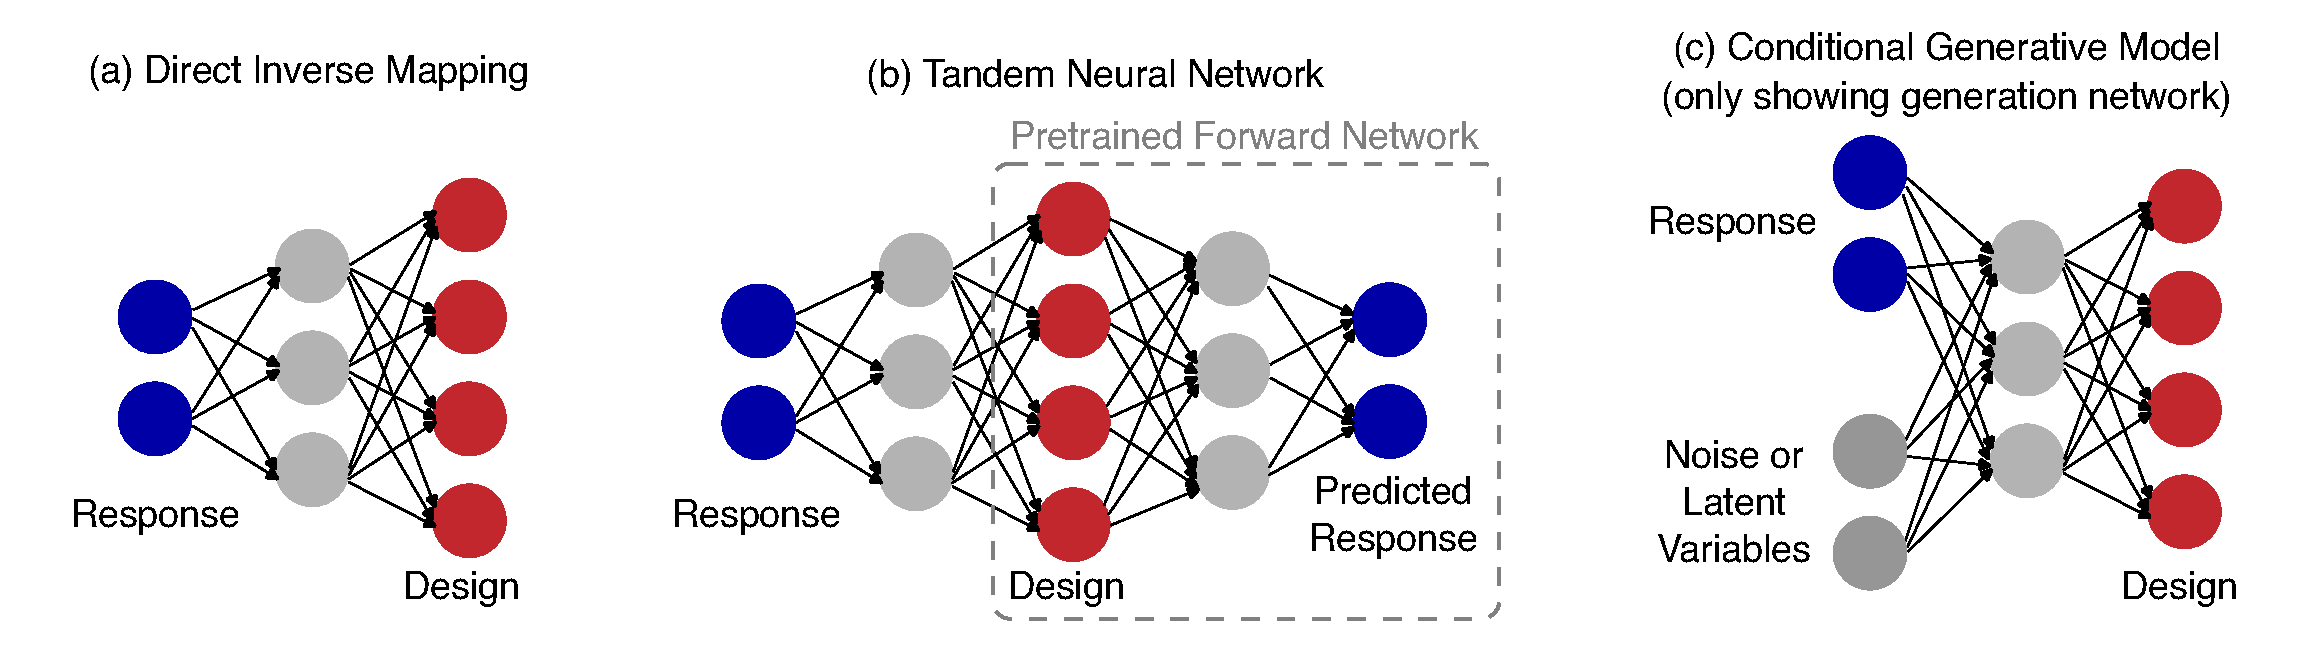
\includegraphics[width=\textwidth]{fig/support_past_work.pdf}
\caption{Three major machine learning models for single-shot inverse design. Note that these are only conceptual plots and the networks can be more complicated in reality. Also, due to the diversity and complexity of conditional generative model architectures, we only show the network for design generation based on commonly used models (e.g., generators in cGANs or decoders in cVAEs), while omitting networks that are necessary for training (e.g., discriminators in cGANs or encoders in cVAEs).}
\label{fig:support_past_work}
\end{figure}


%%%%%%%%%%%%%%%%%%%%%%%%%%%%%%%%%%%%%%%%%%%%%%%
\section{Explanation of Step 2 in RIGID}
\label{sec:app_step2}

The purpose of Step 2 is to obtain the intersection of relevant design space regions for all the ranges of $s$ in a target. We are approximating this goal by simply obtaining the intersection of relevant leaves. However, some non-intersecting leaves may still have intersecting design space regions. When assigning the probability to the intersecting region of two non-intersecting leaves $A$ and $B$, we need to consider the predicted probabilities at both leaves ($P_A$ and $P_B$). Specifically, the assigned probability at this intersecting region should be $P_AP_B$, which can be small. Therefore, we adopt the simplification of only considering the intersection of relevant leaves and ignoring the intersecting regions associated with non-intersecting leaves. The results also demonstrate that this is a reasonable approximation.


%%%%%%%%%%%%%%%%%%%%%%%%%%%%%%%%%%%%%%%%%%%%%%%
\section{Computational Methods for Data Collection and Validation}

\subsection{Computation of Acoustic Dispersion Relations} We performed Bloch-wave analysis in COMSOL Multiphysics to compute the dispersion relations of acoustic metamaterials. Poisson's ratio of 0.49, Young's modulus of 2.7 GPa, and density of 1170 kg/m${^3}$ were set as material properties with $\sim1.5\times10^4$ mesh elements per unit cell. 
We used Floquet-Bloch periodic boundary conditions to obtain the first 60 eigenfrequencies along all symmetry domains of the cubic irreducible Brillouin zone (Fig. \ref{fig:acoustic}B) for all lattices, thus generating a dispersion relation. 

\subsection{Computation of Optical Absorbance Spectra} We computed the absorbance spectra for optical metasurfaces using wave analysis inspired by Zhang et al.~\cite{zhang2023high}. The RF Module of COMSOL Multiphysics\textsuperscript{\textregistered}~\cite{comsol2020} was used to evaluate the spectral response of concern, which is the energy absorbance $A(s)$ in the visible regime (380-700 nm). An absorbance spectrum is computed with respect to 33 wavelength components $s_k$ that are uniformly discretized over the specified range. An incident plane wave is assumed to be given from the port, located at the top face of the analysis domain. We set the periodicity of the analysis domain as 400 nm. The periodic boundary condition on electromagnetic fields is imposed on the lateral faces of the analysis domain. A substrate made of SiO$_2$ is placed right below a given unit cell instance (the black layers in Fig.~\ref{fig:optical}A-B). With full electric fields computed through the wave analysis, the energy absorbance at a single wavelength $s$ is quantified as $A(s)=1-|S_{11}(s)|^2$, where $S_{ij}$ is the component of the $S$-parameter matrix that specifies energy transfer between ports. We use the data presented in Ref.~\cite{aspnes1983dielectric} to set the material dispersion of the dielectric.





%%%%%%%%%%%%%%%%%%%%%%%%%%%%%%%%%%%%%%%%%%%%%%%
\section{Test performance of forward prediction}

Test data for all the design problems are designs $\mathbf{x}$ (that the random forests have never seen during training) and their corresponding qualitative behaviors $y\in\{0,1\}$ based on functional responses.

In the acoustic metamaterial design problem, we have 57 test designs, yielding 5,700 test points as the entire frequency range of dispersion relations is discretized into 100 intervals for each design. In the optical metasurface design problem, we have 52 test designs, with each functional response discretized into 33 points, which yields 1,716 test points in total. In each of the synthetic design problems, we have 20 synthetic test designs, with each synthetic response discretized into 100 points. This results in 2,000 test data points in total. Confusion matrices showing test performances are in Tables~\ref{tab:f1_acoustic}-\ref{tab:f1_test_func_sin}.

\begin{table}[h]
\caption{Confusion matrix on test data in the acoustic metamaterial design problem. The test F1 score is 0.82.}
\centering
\makegapedcells
\begin{tabular}{cc|cc}
\multicolumn{2}{c}{}
            &   \multicolumn{2}{c}{Predicted} \\
    &       &   Yes &   No              \\ 
    \cline{2-4}
\multirow{2}{*}{\rotatebox[origin=c]{90}{Actual}}
    & Yes   & 393   & 131                 \\
    & No    & 46    & 5130                \\ 
    \cline{2-4}
    \end{tabular}
\label{tab:f1_acoustic}
\end{table}



\begin{table}[h]
\caption{Confusion matrix on test data in the optical metasurface design problem. The test F1 score is 0.83.}
\centering
\makegapedcells
\begin{tabular}{cc|cc}
\multicolumn{2}{c}{}
            &   \multicolumn{2}{c}{Predicted} \\
    &       &   Yes &   No              \\ 
    \cline{2-4}
\multirow{2}{*}{\rotatebox[origin=c]{90}{Actual}}
    & Yes   & 776   & 157                 \\
    & No    & 151    & 632                \\ 
    \cline{2-4}
    \end{tabular}
\label{tab:f1_optical}
\end{table}




\begin{table}[h]
\caption{Confusion matrix on test data in the SqExp problem. The test F1 score is 0.85.}
\centering
\makegapedcells
\begin{tabular}{cc|cc}
\multicolumn{2}{c}{}
            &   \multicolumn{2}{c}{Predicted} \\
    &       &   Yes &   No              \\ 
    \cline{2-4}
\multirow{2}{*}{\rotatebox[origin=c]{90}{Actual}}
    & Yes   & 229   & 68                 \\
    & No    & 13    & 1690                \\ 
    \cline{2-4}
    \end{tabular}
\label{tab:f1_test_func_sqexp}
\end{table}



\begin{table}[h]
\caption{Confusion matrix on test data in the SupSin problem. The test F1 score is 0.86.}
\centering
\makegapedcells
\begin{tabular}{cc|cc}
\multicolumn{2}{c}{}
            &   \multicolumn{2}{c}{Predicted} \\
    &       &   Yes &   No              \\ 
    \cline{2-4}
\multirow{2}{*}{\rotatebox[origin=c]{90}{Actual}}
    & Yes   & 355   & 81                 \\
    & No    & 37    & 1527                \\ 
    \cline{2-4}
    \end{tabular}
\label{tab:f1_test_func_sin}
\end{table}




%%%%%%%%%%%%%%%%%%%%%%%%%%%%%%%%%%%%%%%%%%%%%%%
\section{Generated Designs and Corresponding Responses}

Figures~\ref{fig:support_acoustic_1}-\ref{fig:support_optical_2} show the rest of generated designs and their corresponding responses in addition to those in Figures~\ref{fig:acoustic}F and \ref{fig:optical}F.


\begin{figure}
\centering
\includegraphics[width=\textwidth]{fig/support_acoustic_1.pdf}
\caption{Geometries and corresponding dispersion relations of generated acoustic metamaterial designs for bandgap targets \rom{2}-\rom{4} (marked as gray-shaded frequency regions). Each row shows five designs with the highest likelihood of satisfying a target. 
% The number below each geometry indicates the corresponding estimated likelihood value.
}
\label{fig:support_acoustic_1}
\end{figure}

\begin{figure}
\centering
\includegraphics[width=\textwidth]{fig/support_acoustic_2.pdf}
\caption{Geometries and corresponding dispersion relations of generated acoustic metamaterial designs for bandgap targets \rom{5}-\rom{7} (marked as gray-shaded frequency regions). Each row shows five designs with the highest likelihood of satisfying a target. 
% The number below each geometry indicates the corresponding estimated likelihood value.
}
\label{fig:support_acoustic_2}
\end{figure}

\begin{figure}
\centering
\includegraphics[width=\textwidth]{fig/support_acoustic_3.pdf}
\caption{Geometries and corresponding dispersion relations of generated acoustic metamaterial designs for bandgap targets \rom{8}-\rom{10} (marked as gray-shaded frequency regions). Each row shows five designs with the highest likelihood of satisfying a target. 
% The number below each geometry indicates the corresponding estimated likelihood value.
}
\label{fig:support_acoustic_3}
\end{figure}

\begin{figure}
\centering
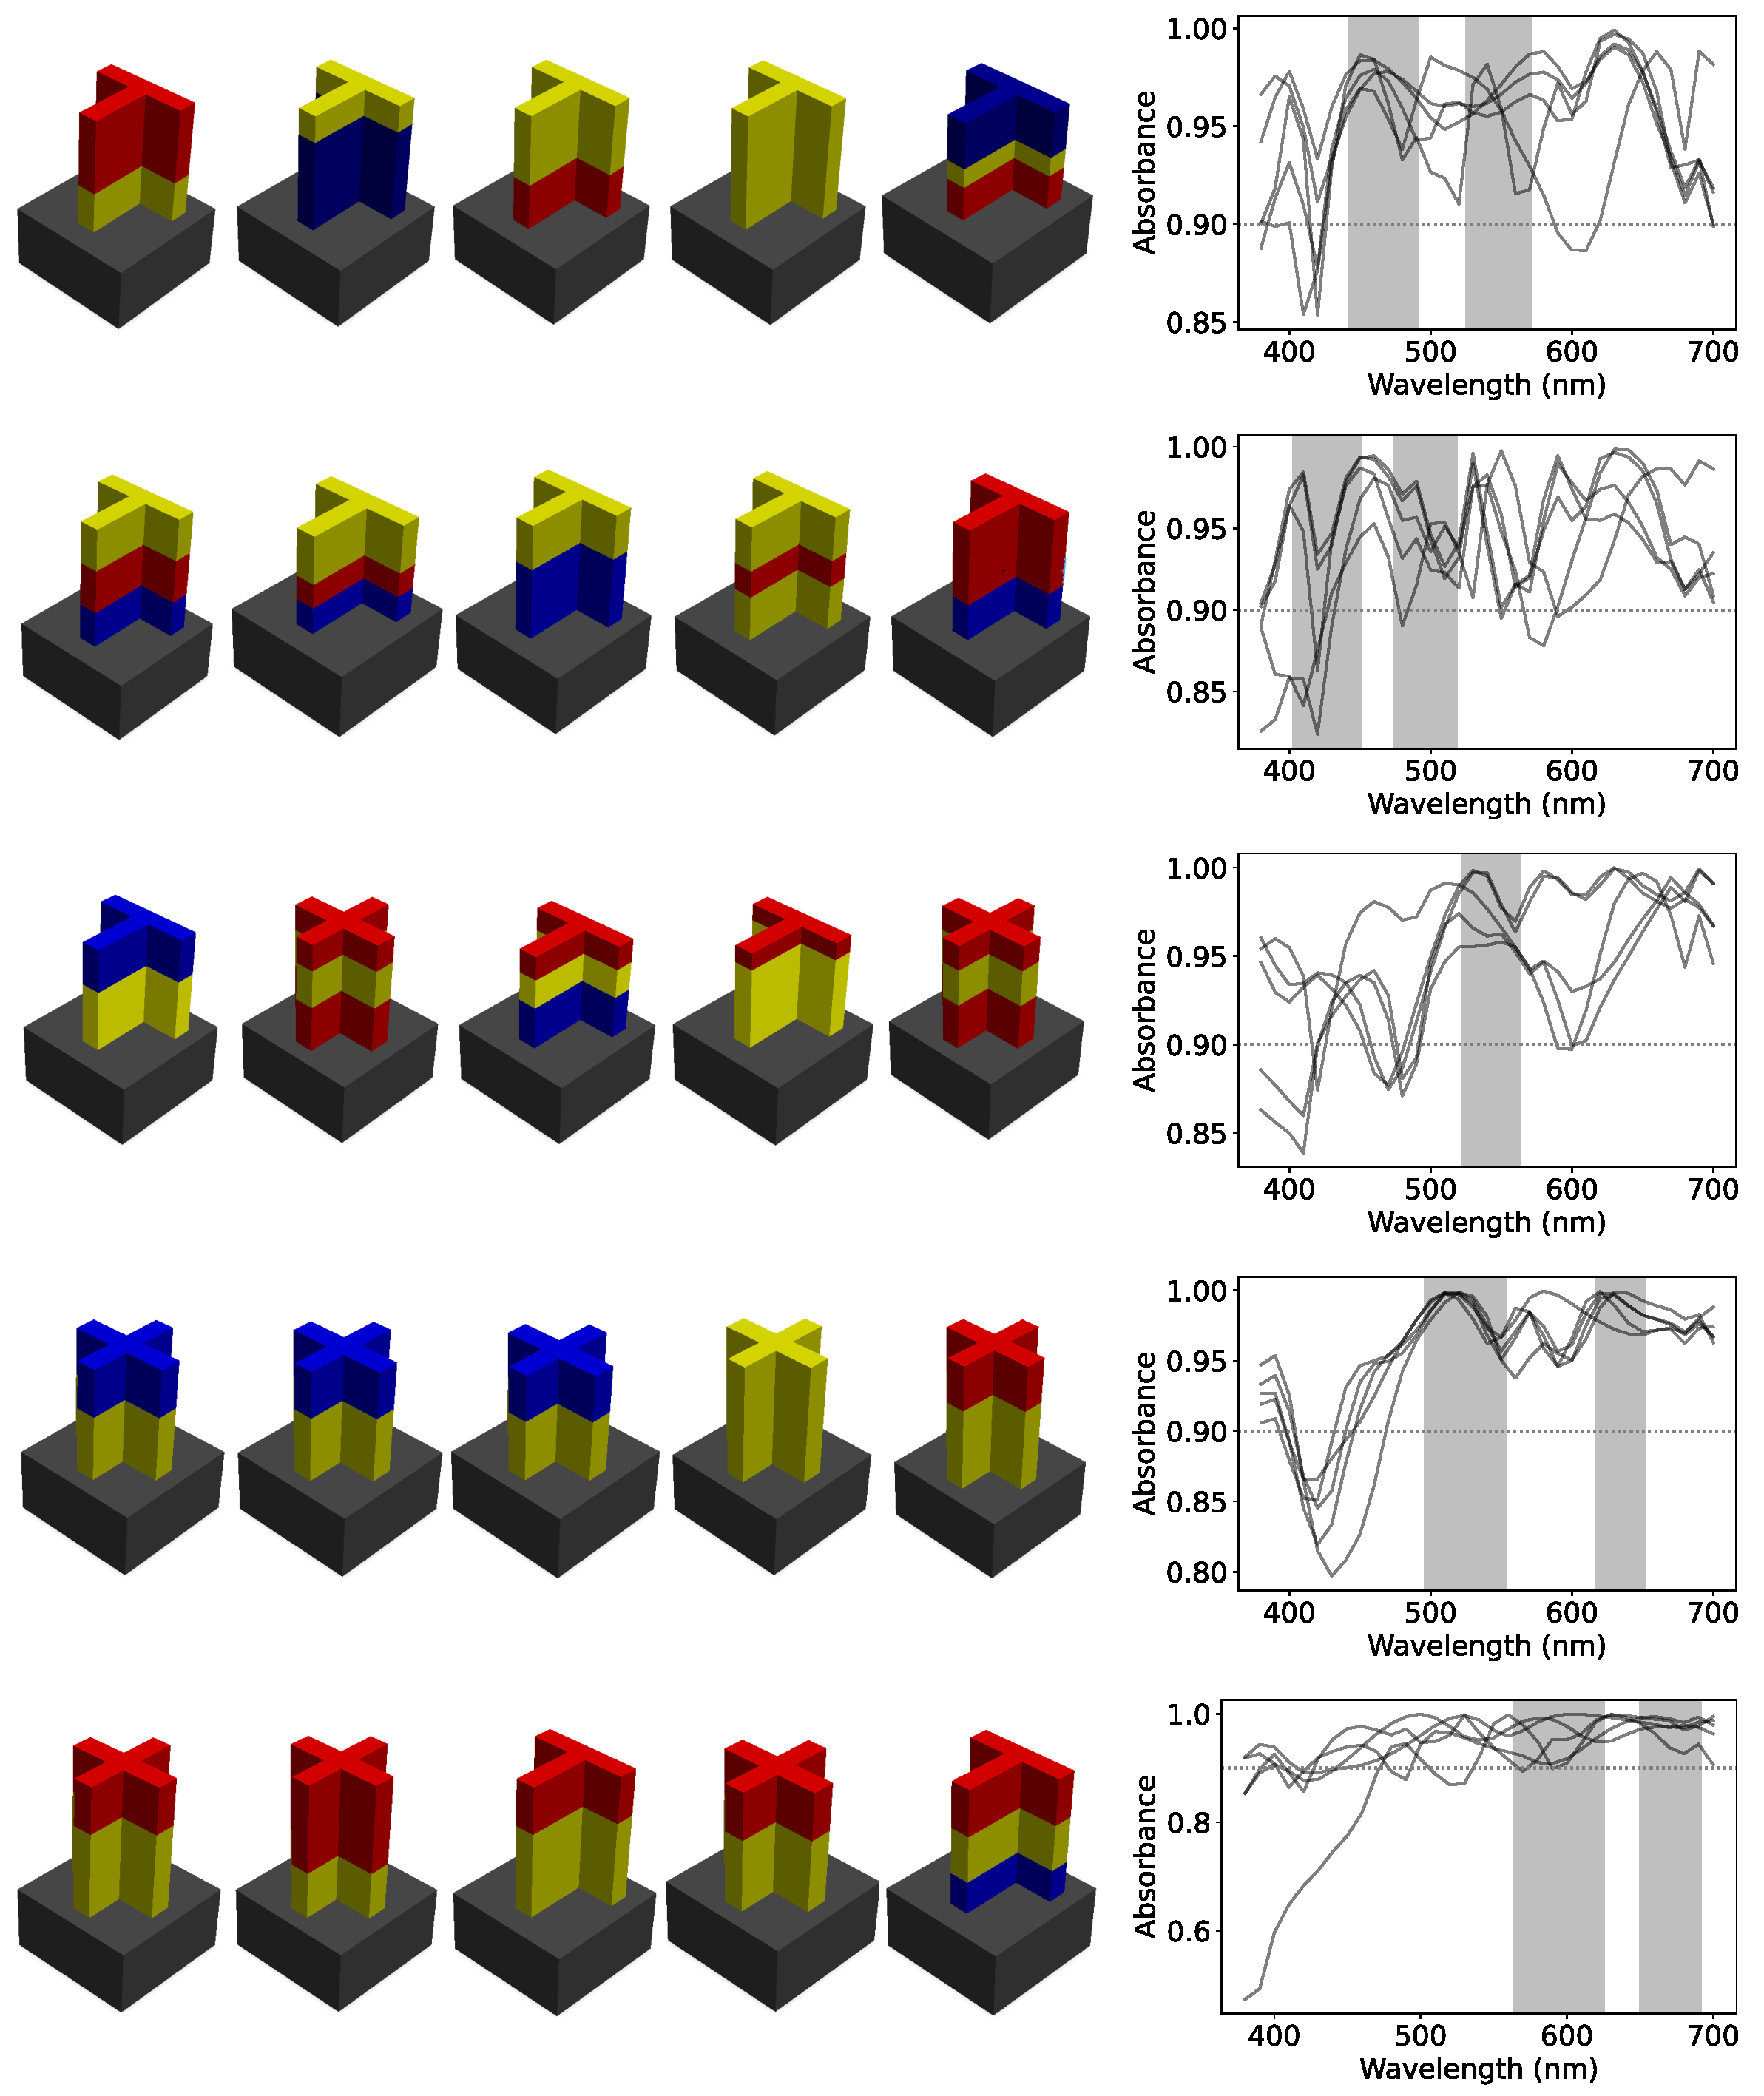
\includegraphics[width=\textwidth]{fig/support_optical_1.pdf}
\caption{Designs and corresponding absorbance spectra of generated optical metasurface designs for design targets \rom{2}-\rom{6} (marked as gray-shaded wavelength regions). Each row shows five designs with the highest likelihood of satisfying a target (left panel) and their absorbance spectra (right panel). 
% The number below each design indicates the corresponding estimated likelihood value.
}
\label{fig:support_optical_1}
\end{figure}

\begin{figure}
\centering
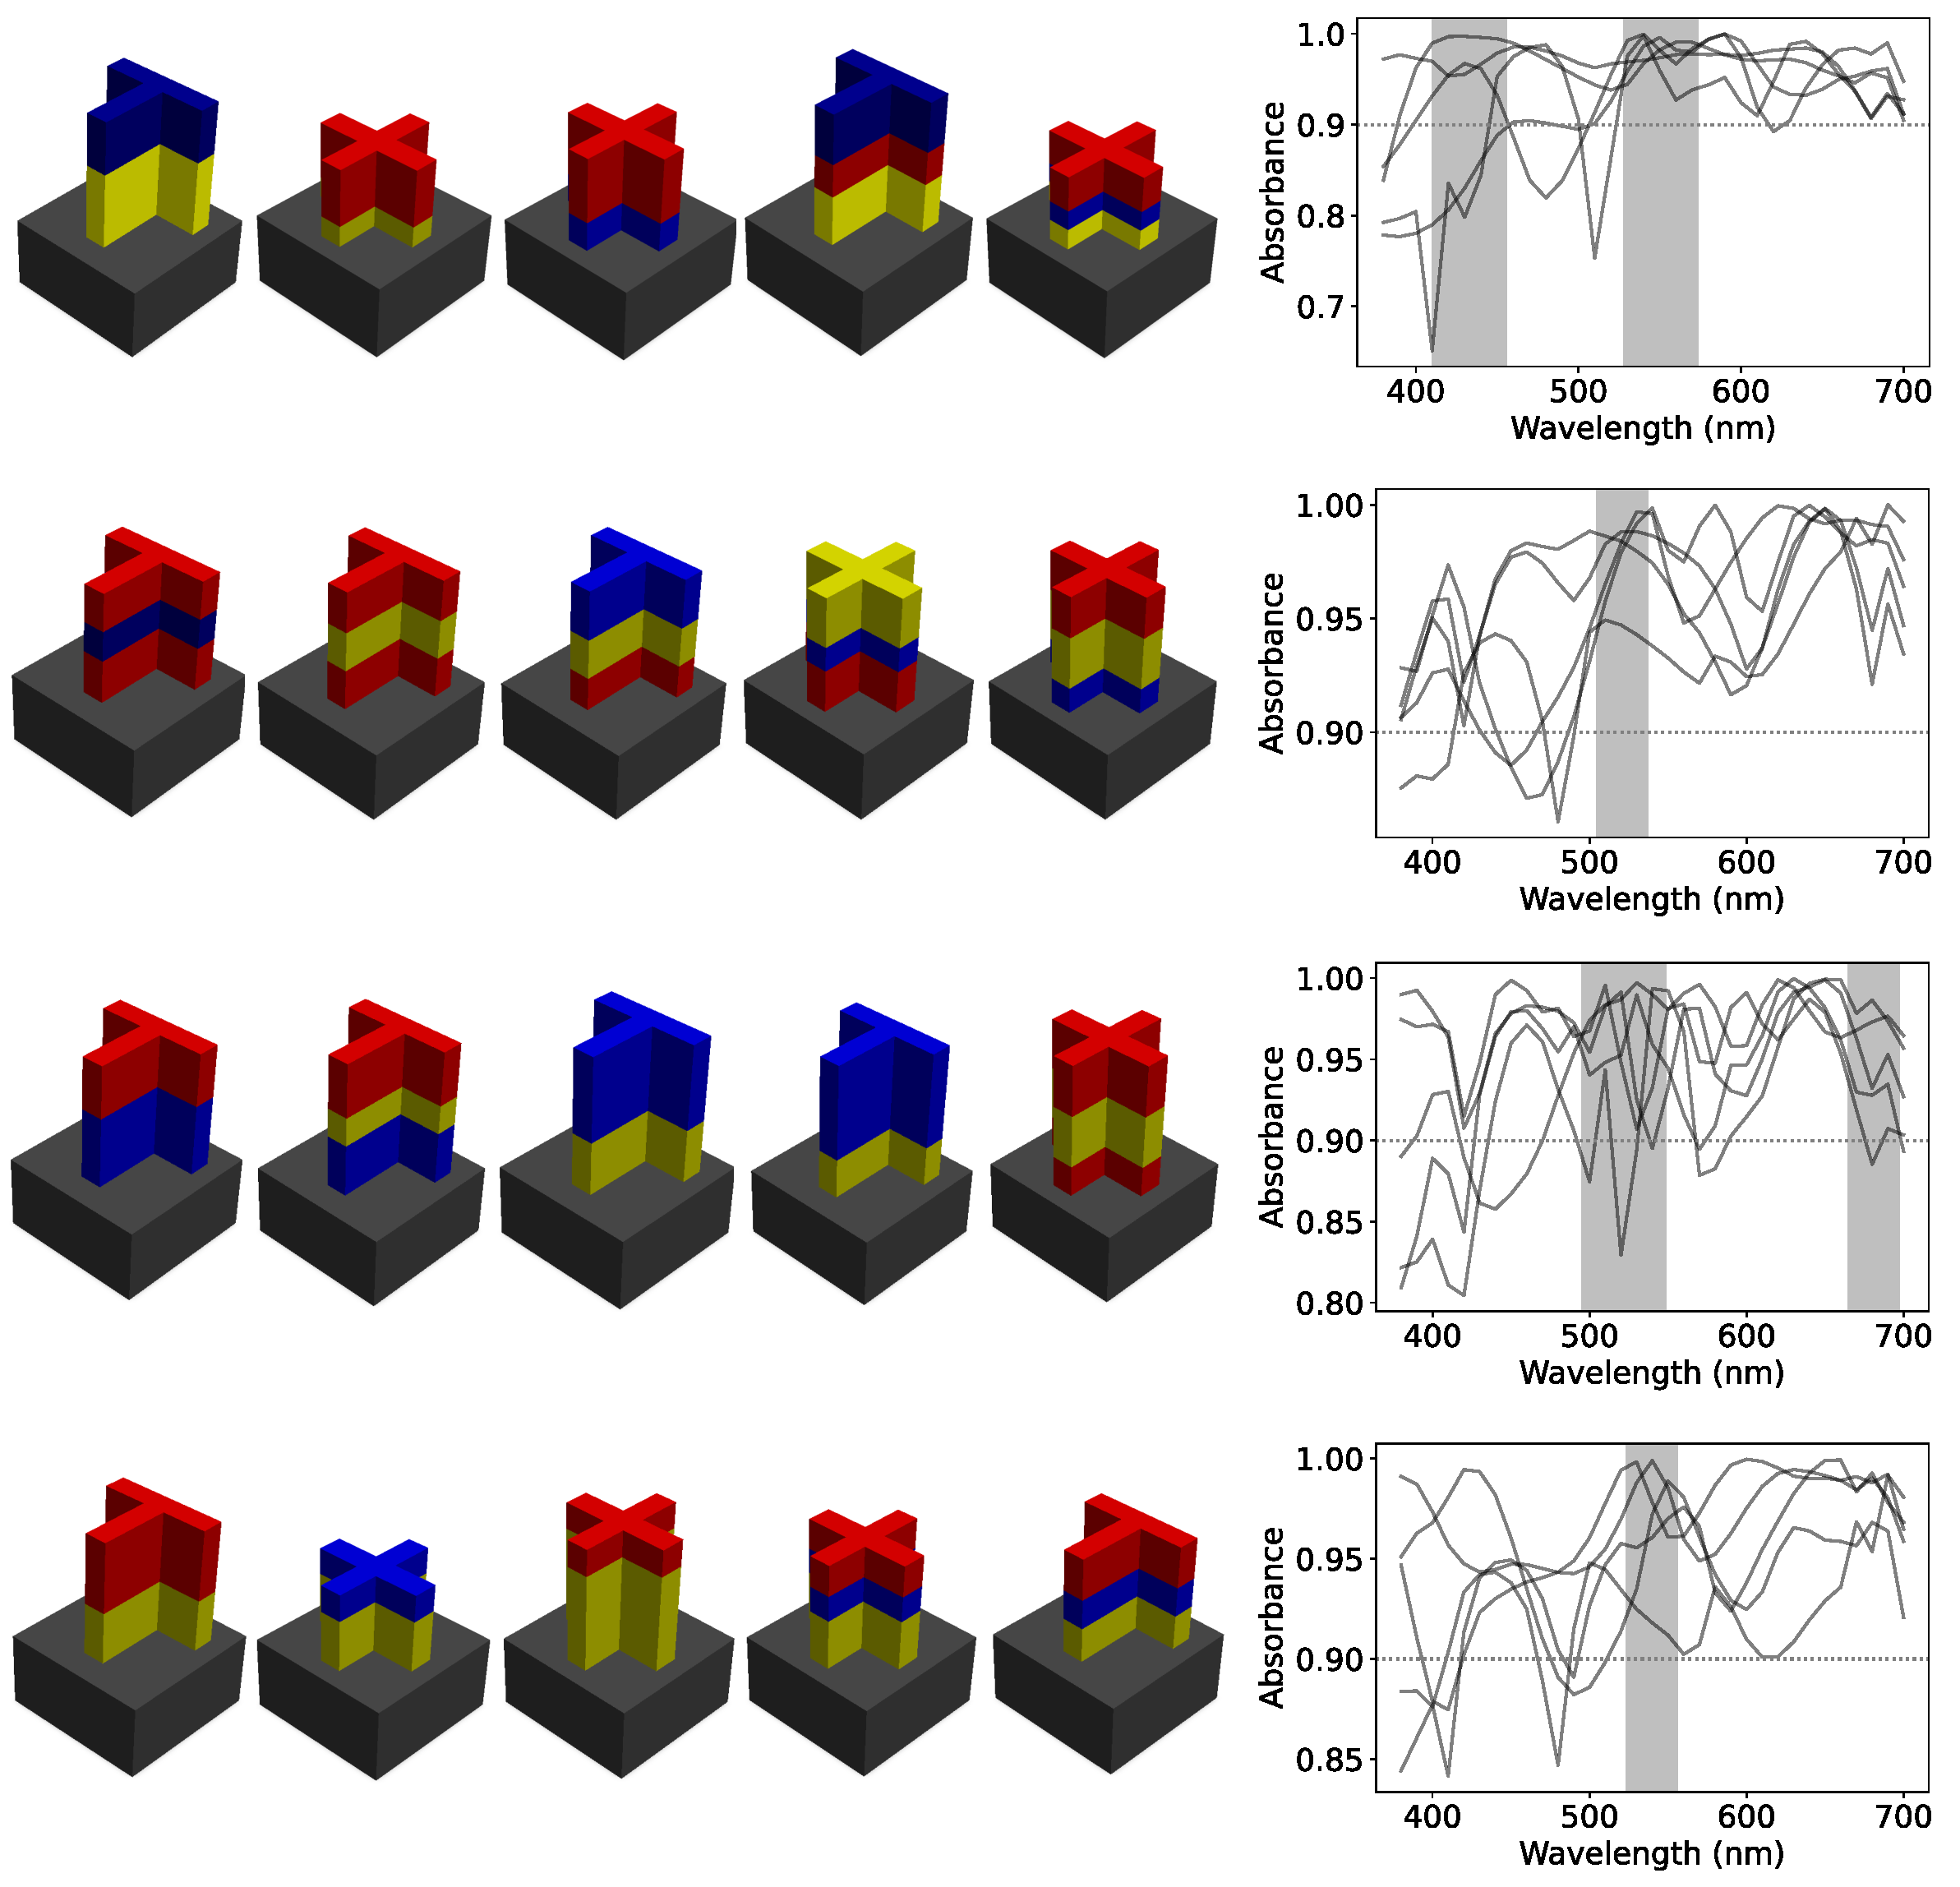
\includegraphics[width=\textwidth]{fig/support_optical_2.pdf}
\caption{Designs and corresponding absorbance spectra of generated optical metasurface designs for design targets \rom{7}-\rom{10} (marked as gray-shaded wavelength regions). Each row shows five designs with the highest likelihood of satisfying a target (left panel) and their absorbance spectra (right panel). 
% The number below each design indicates the corresponding estimated likelihood value.
}
\label{fig:support_optical_2}
\end{figure}



\end{appendices}


\end{document}
